\chapter{Invisible Z Background}
\label{chap:zinv}

One of the main sources of backgrounds to the \mttwo analysis comes from the production of a $Z$
boson in association with one or more jets, where the $Z$ decays ``invisibly'' to two neutrinos.
This is an \emph{irriducible} background, since the signature is exactly like that of signal:
no prompt charged leptons, real \ptmiss, and multiple jets. For signal models that produce
b quarks, however, the number of b-tagged jets becomes a discriminating variable as there are
no inherent b jets in \zjets production.

To estimate this background in a data-driven way, we make use of the fact that $Z$ bosons may also decay into two
charged leptons with known branching fraction. The rate of \zll production is measured in data, and this is
translated into an estimate on \znunu by multiplying by a transfer factor derived from Monte Carlo.
Section~\ref{sec:znunu_from_zll} describes how this is done in each $(\Ht,\Nj,\Nb)$ topological region,
Sec.~\ref{sec:zinv_mt2} details the ``hybrid template'' method for extrapolating the estimate along the
\mttwo dimension, and Sec.~\ref{sec:zinv_syst} describes the systematic uncertainties assessed on the 
final estimate.

\section{Estimating \texorpdfstring{\znunu}{Z\unichar{"2192}\unichar{"03BD}\unichar{"03BD}} from \texorpdfstring{\zll}{Z\unichar{"2192}ll}}
\label{sec:znunu_from_zll}
The exact definition of the dilepton control region used in the \znunu estimate is described in Sec.~\ref{sec:dilep_cr}.
It is constructed to be enriched in \zll events (as opposed to other dilepton-producing processes, such as \ttbar),
and the lepton \vSS{p}{T}{} vectors are added to the \vMet in order to mimic the kinematics of \znunu events.

Data vs.\ MC comparisons of the main analysis kinematic variables in the baseline \zll control region are 
shown in Fig.~\ref{fig:zll_crplots}. There is some level of disagreement between data and MC, but this is
to be expected. The estimate is primarily data-driven, and MC is used only at leading order, so these
disagreements generally do not affect the final estimate. Where MC is used, primarily in the far
\mttwo tails, appropriate systematic uncertainties are assigned.

\begin{figure}[htbp]
  \begin{center}
    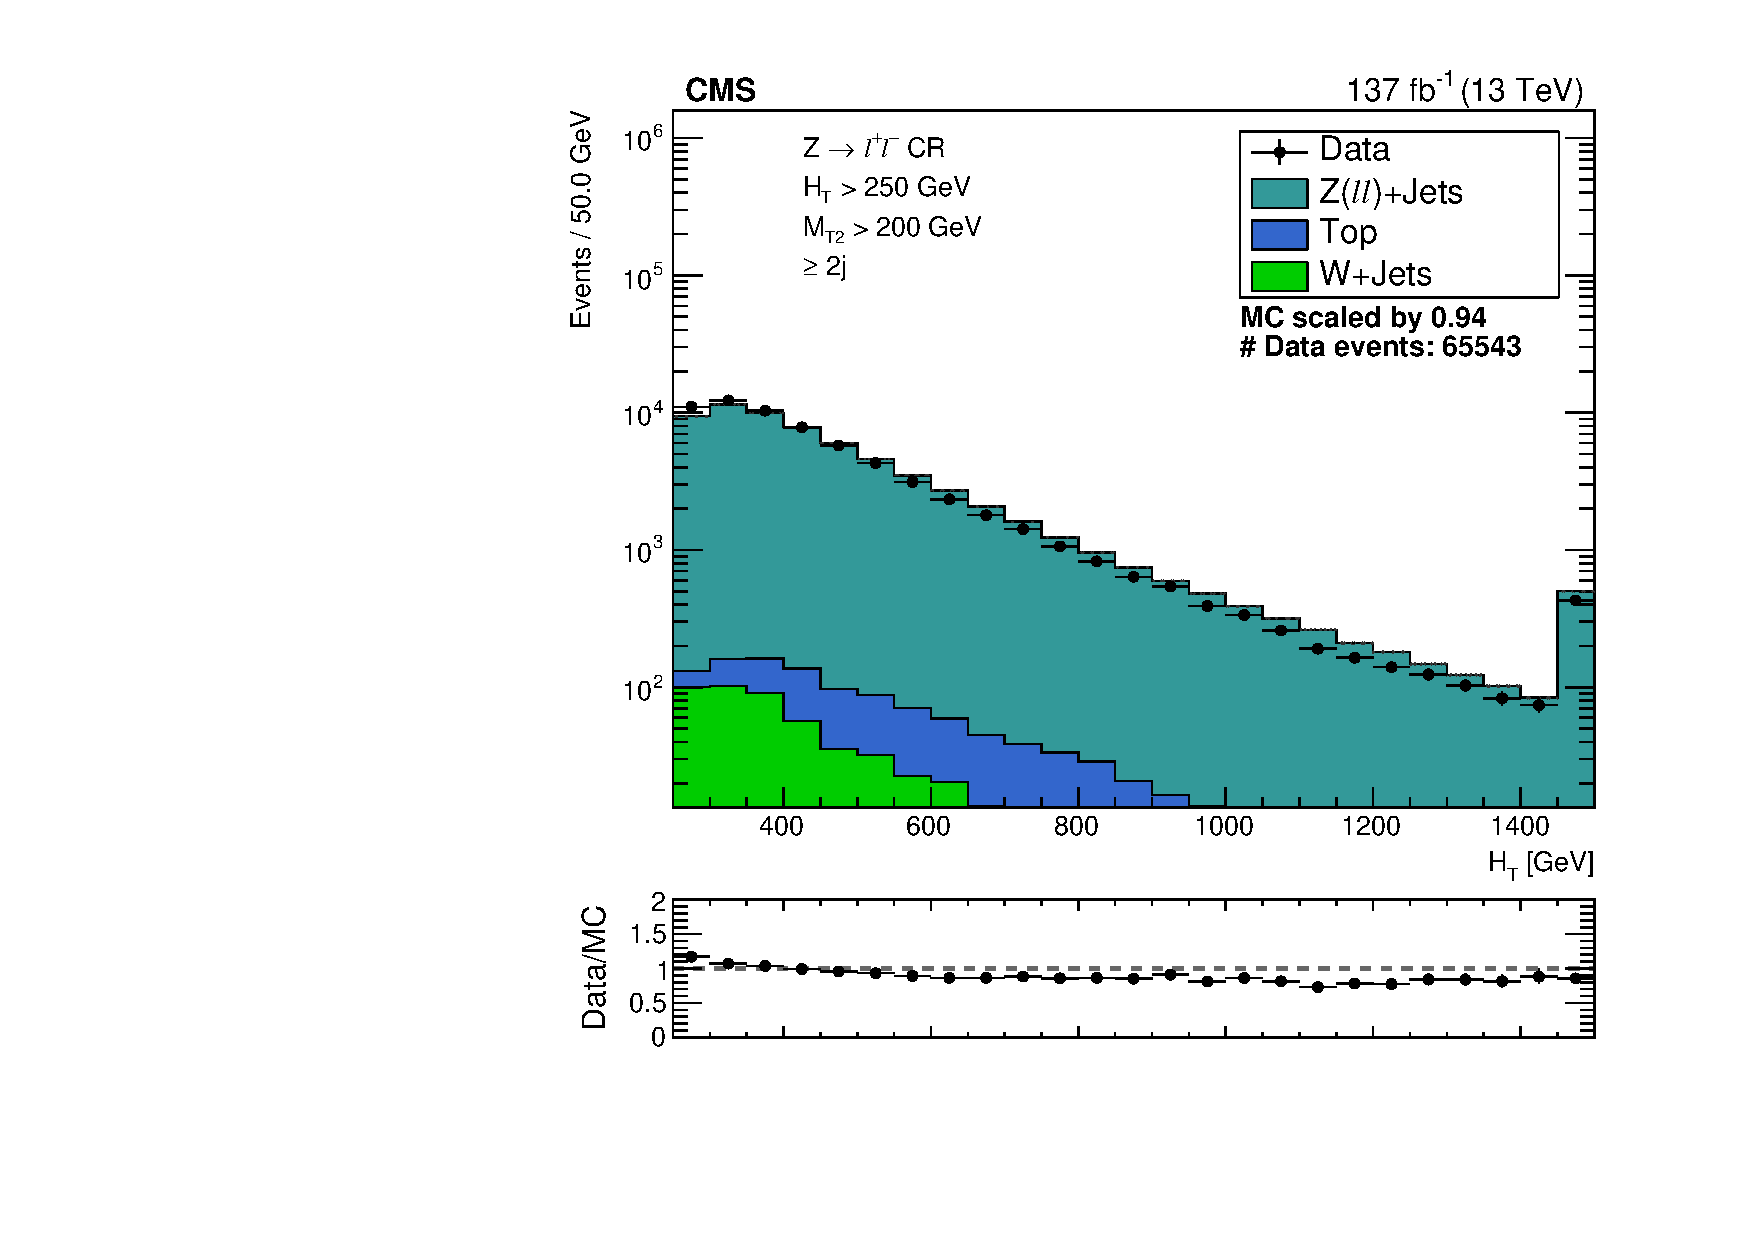
\includegraphics[width=0.47\textwidth]{figs/zinv/crdybase_ht.pdf}
    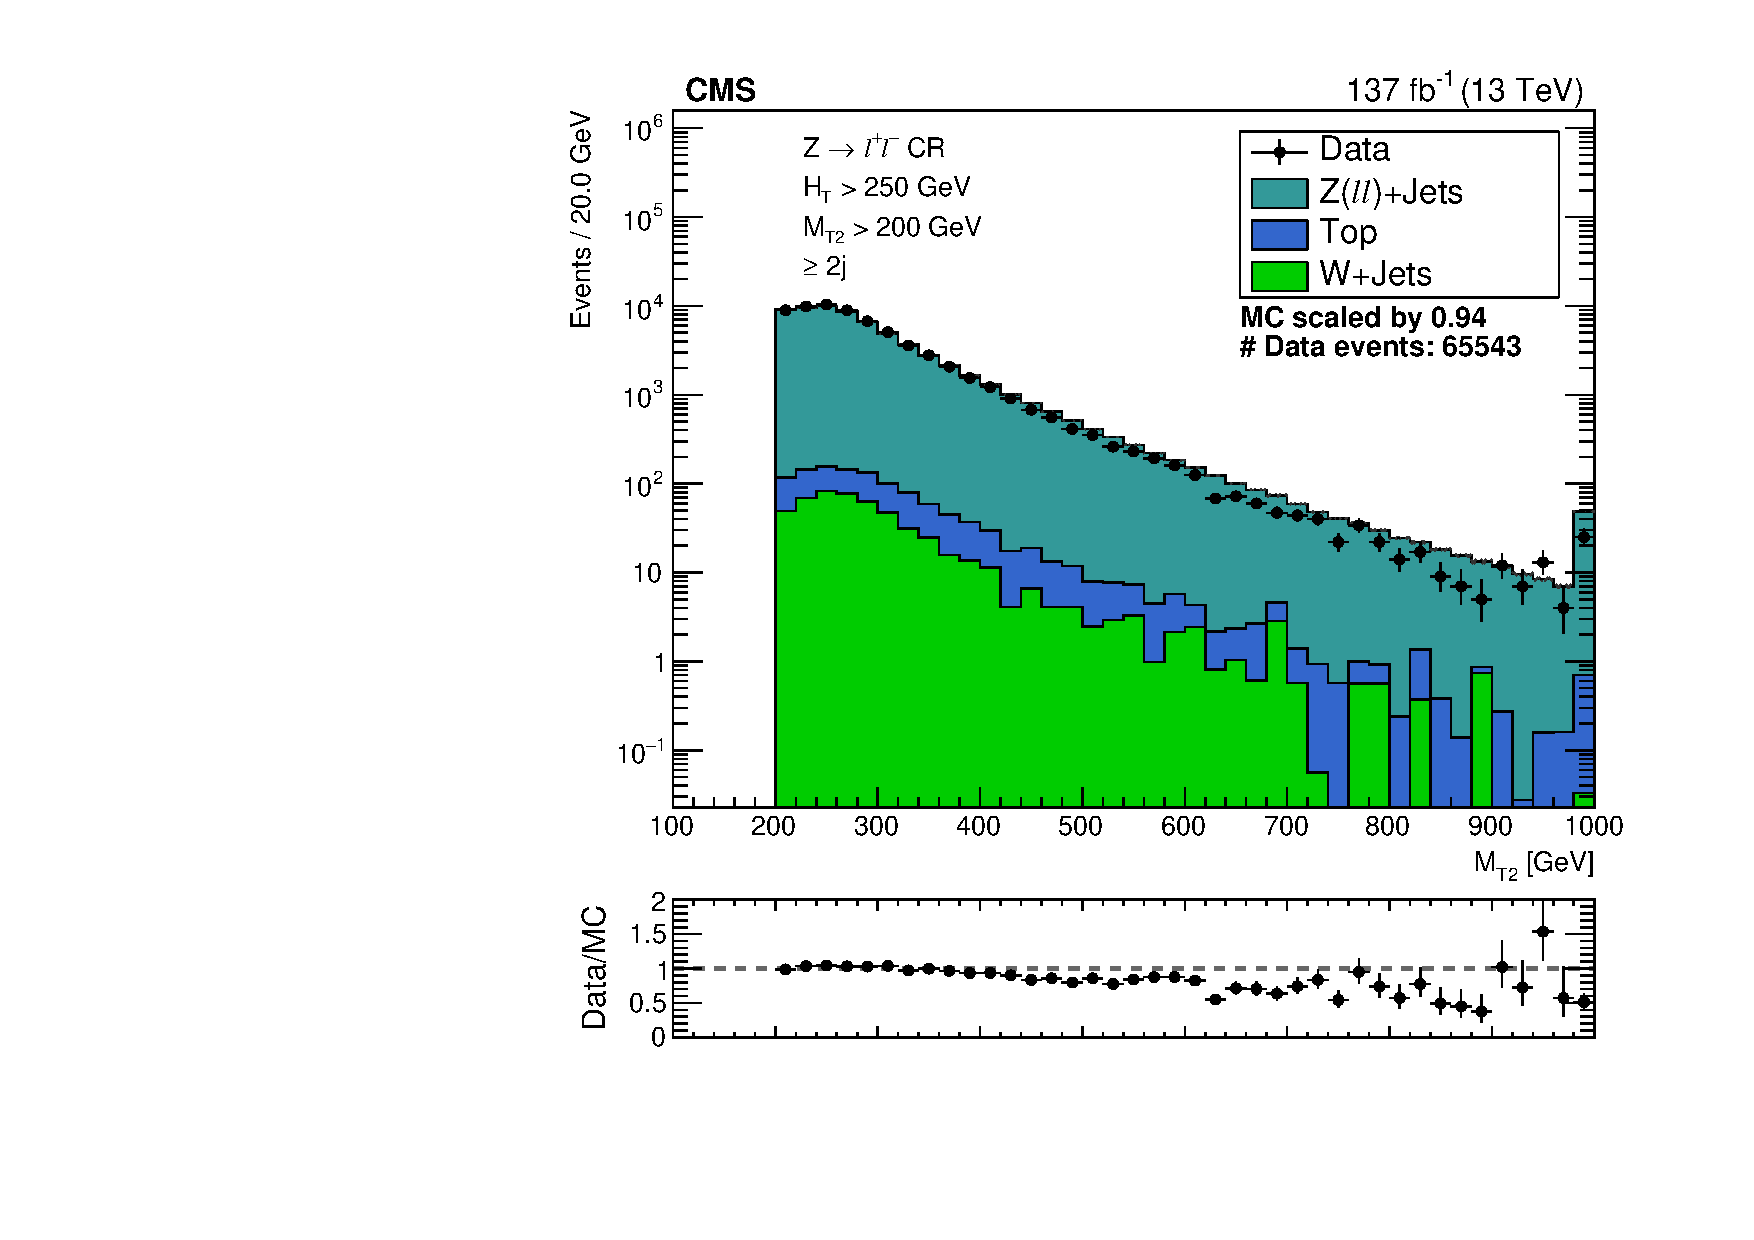
\includegraphics[width=0.47\textwidth]{figs/zinv/crdybase_mt2.pdf} \\
    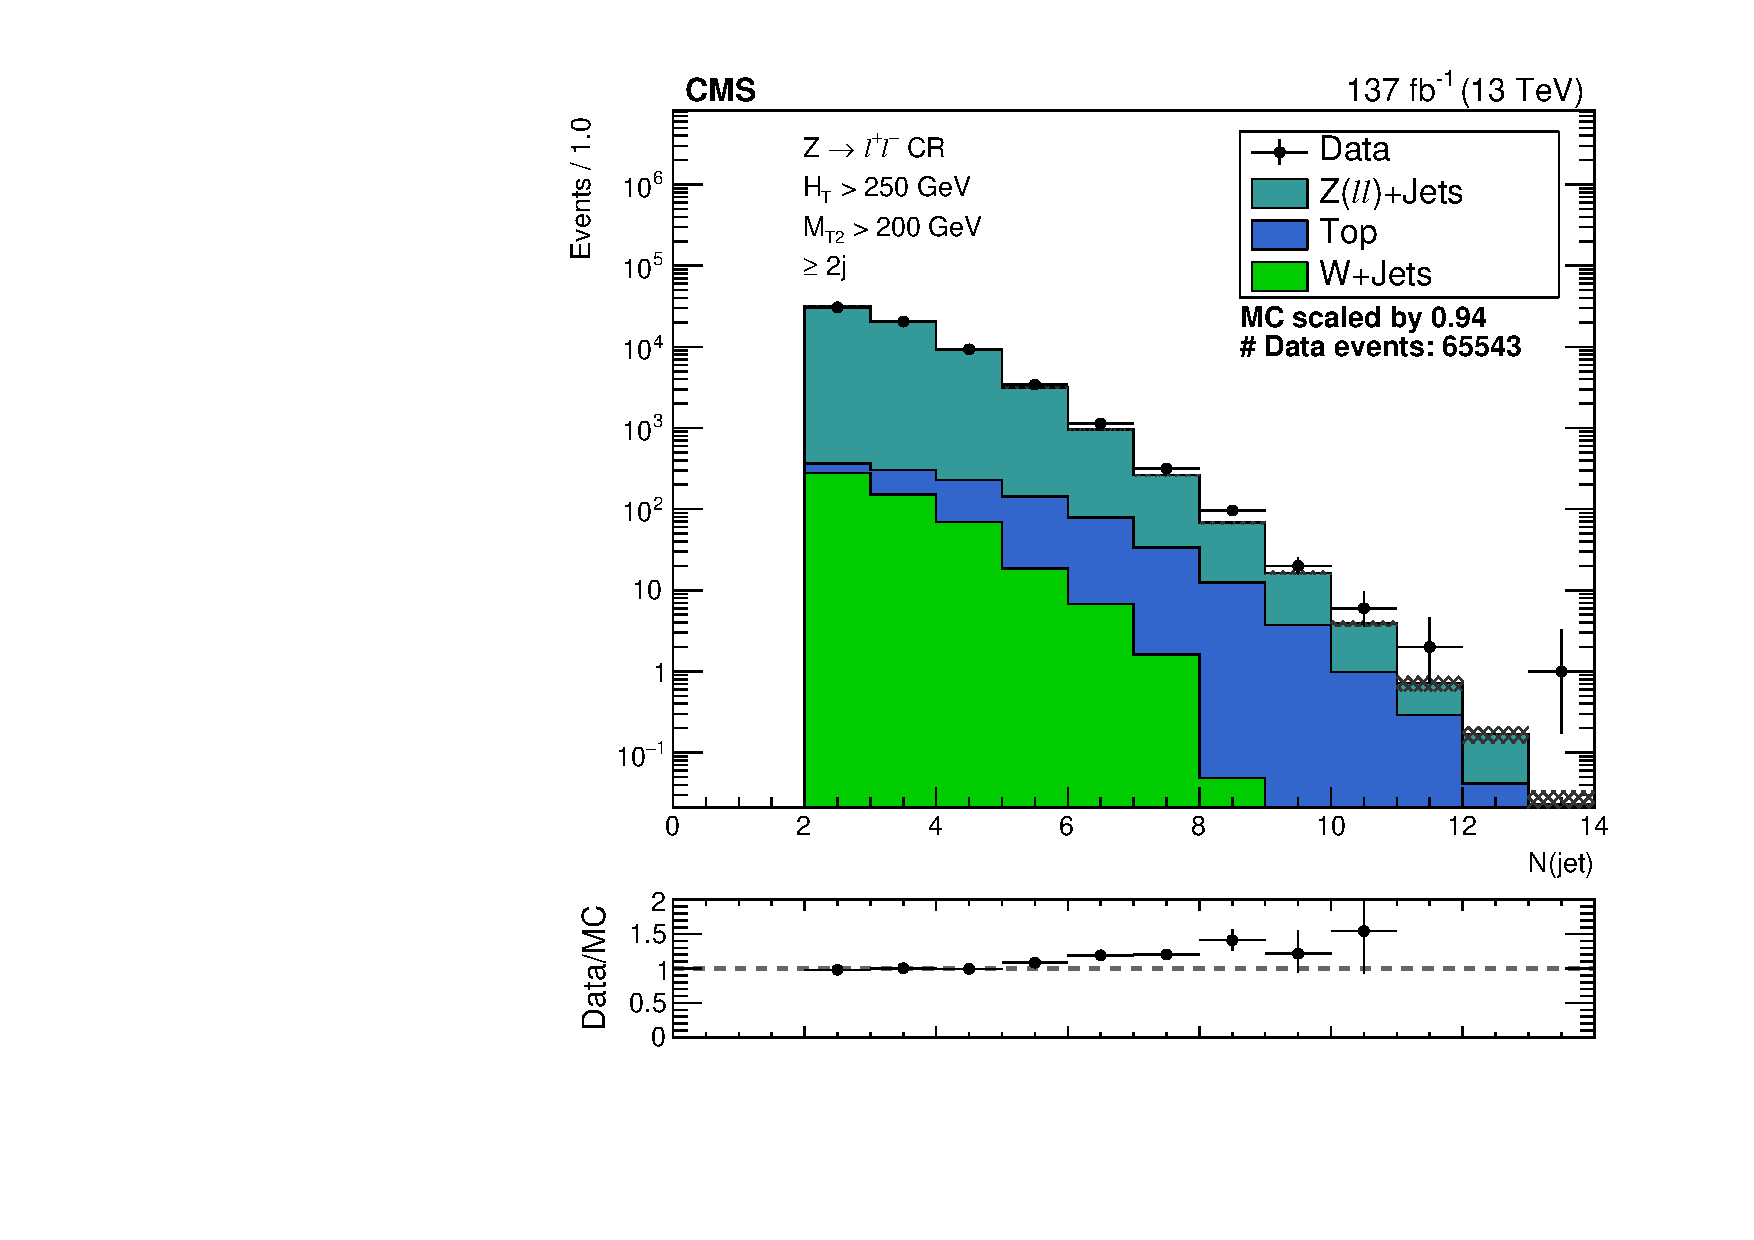
\includegraphics[width=0.47\textwidth]{figs/zinv/crdybase_nJet30.pdf}
    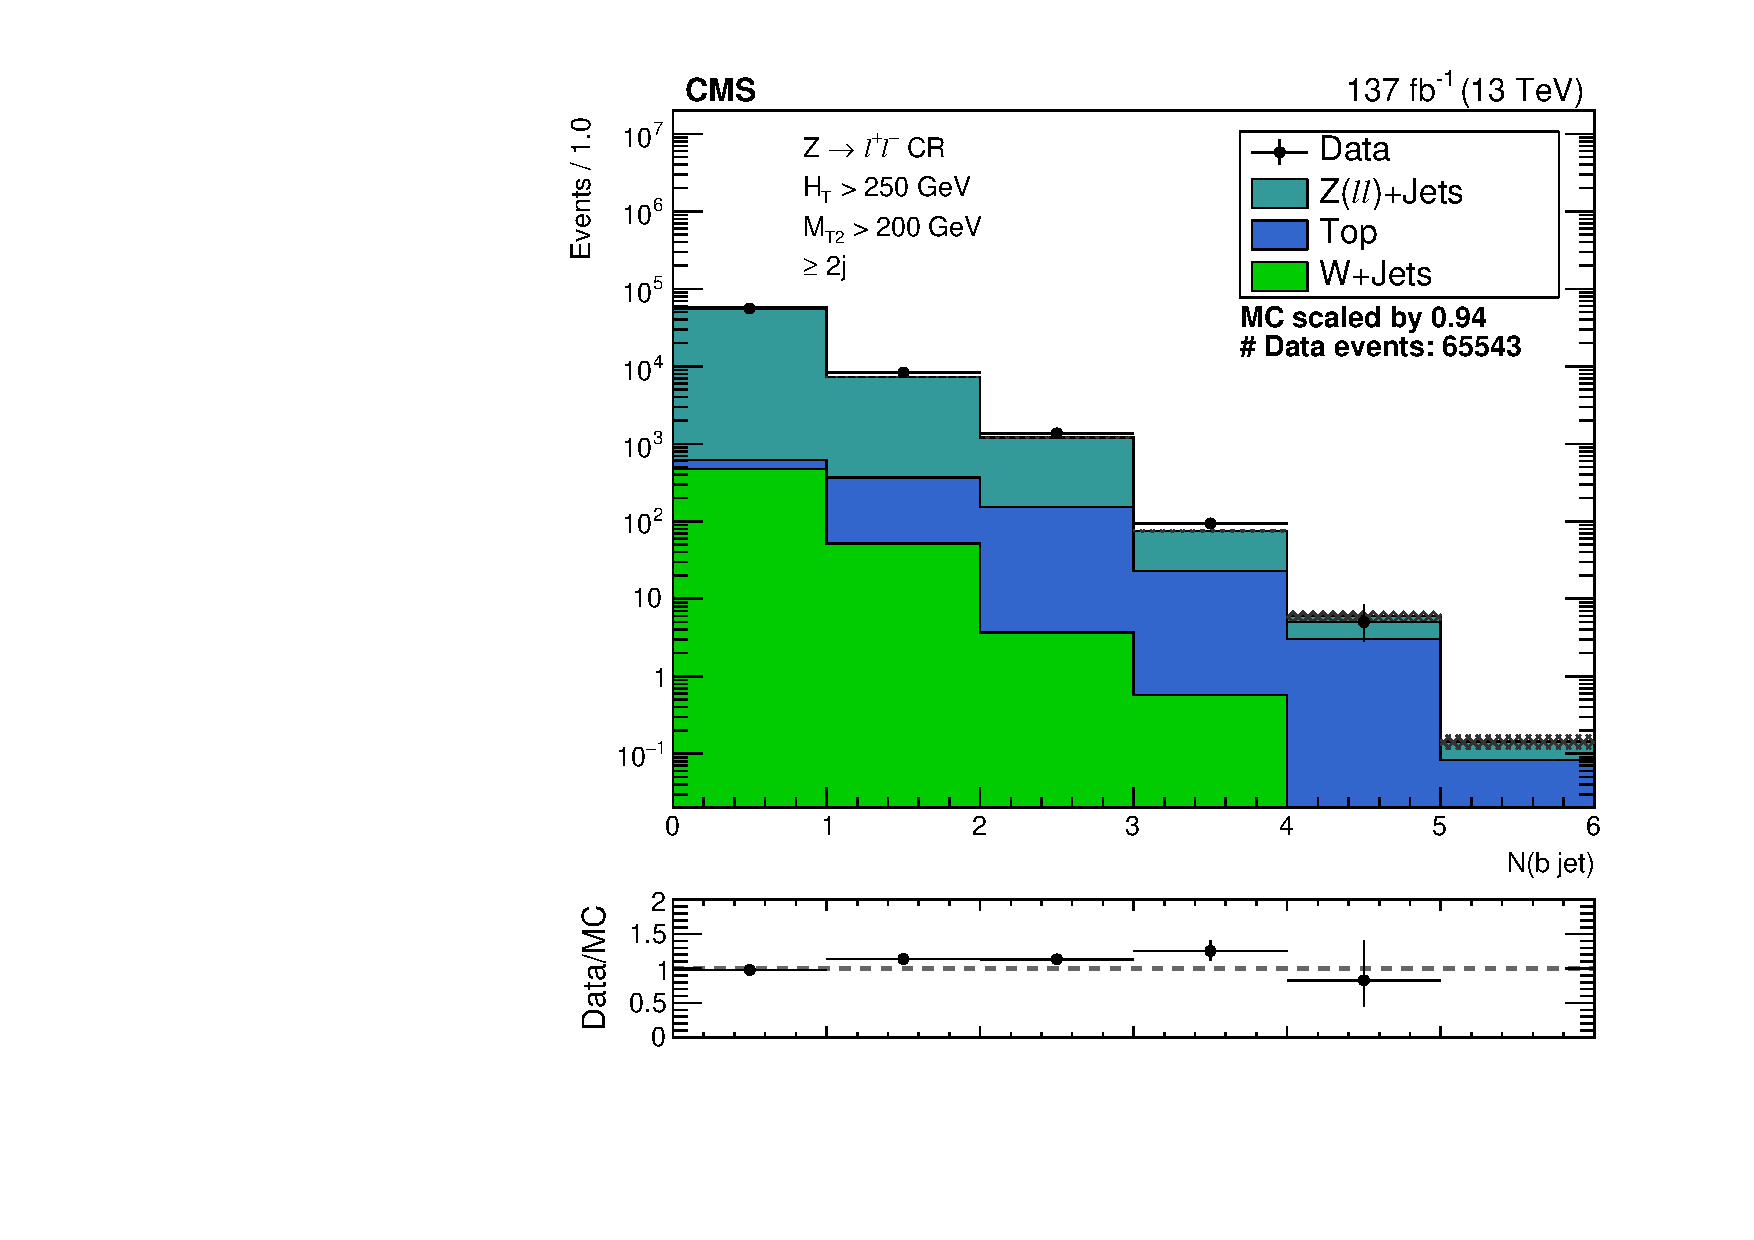
\includegraphics[width=0.47\textwidth]{figs/zinv/crdybase_nBJet20.pdf} \\
    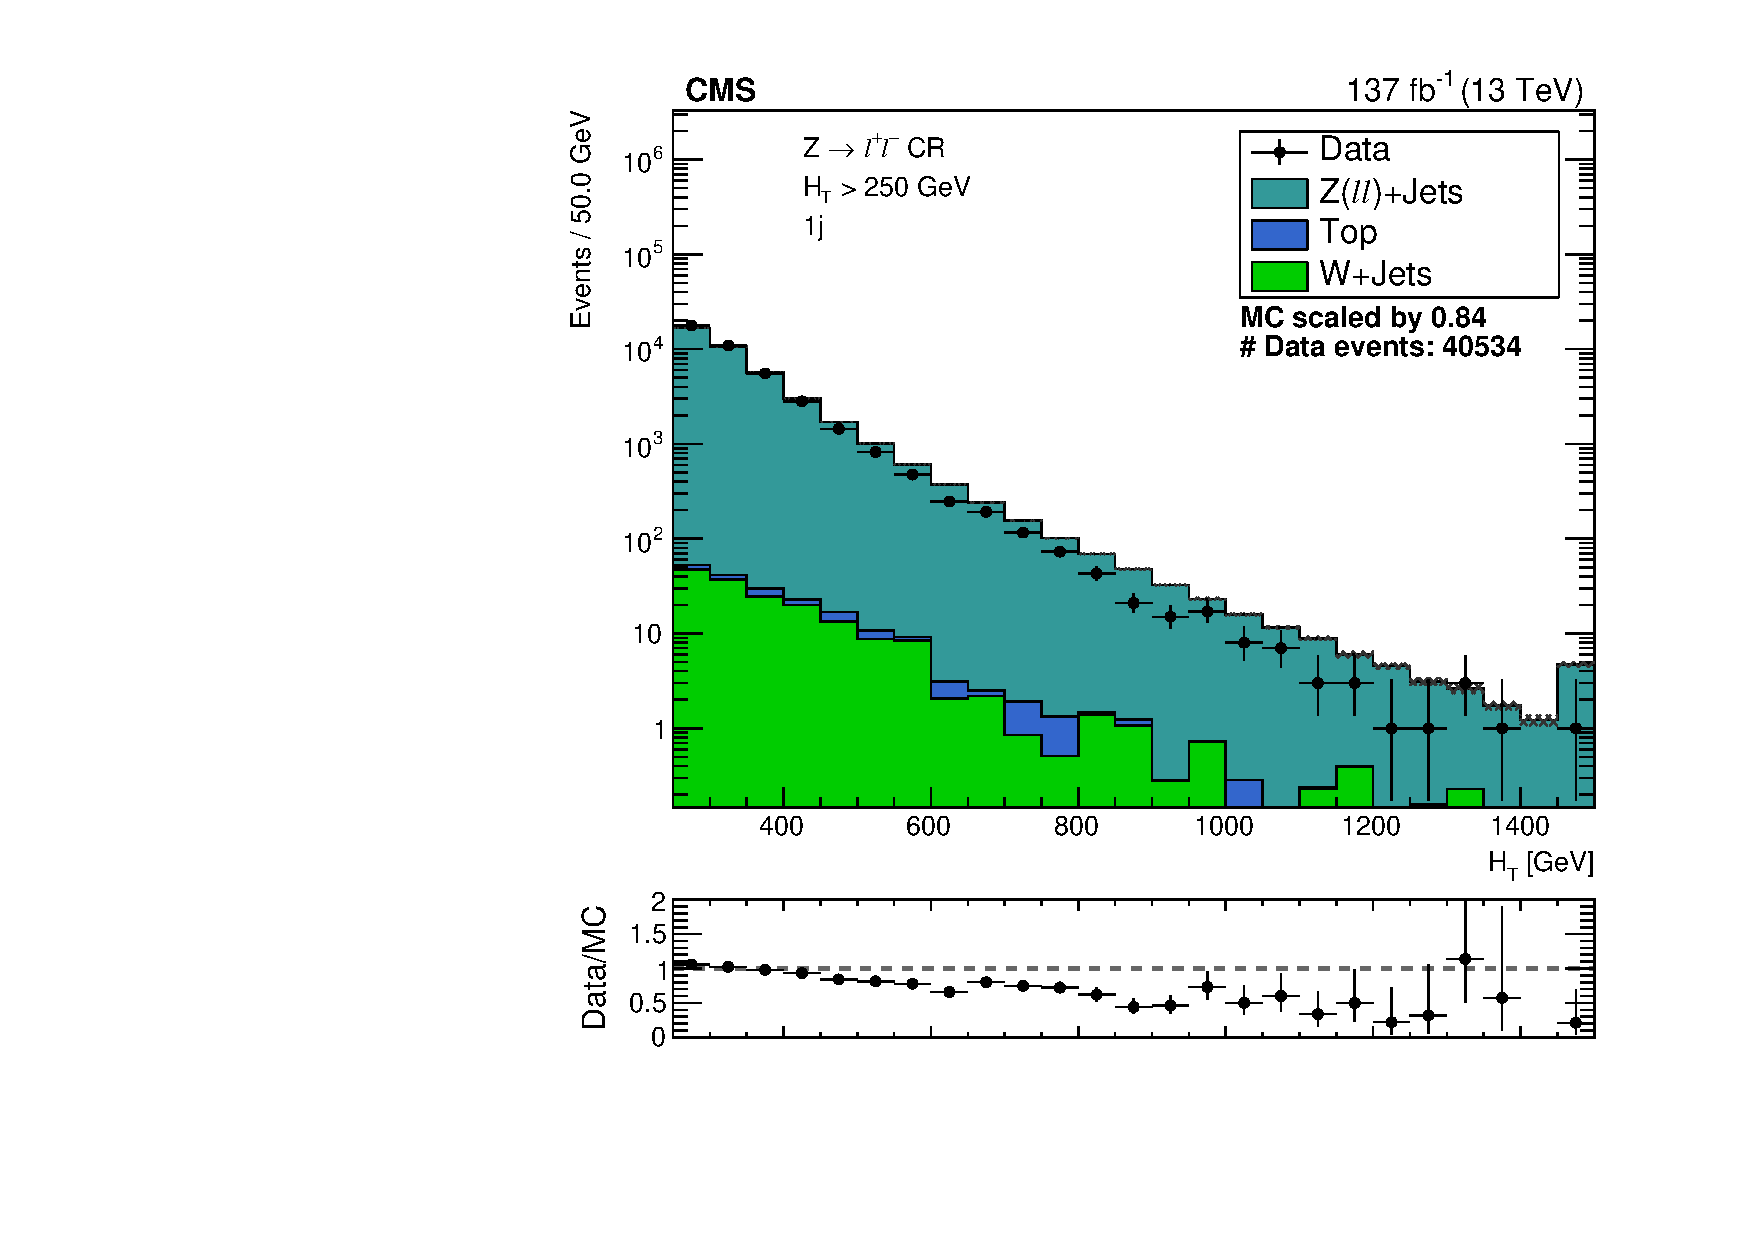
\includegraphics[width=0.47\textwidth]{figs/zinv/crdybaseJ_ht.pdf}
    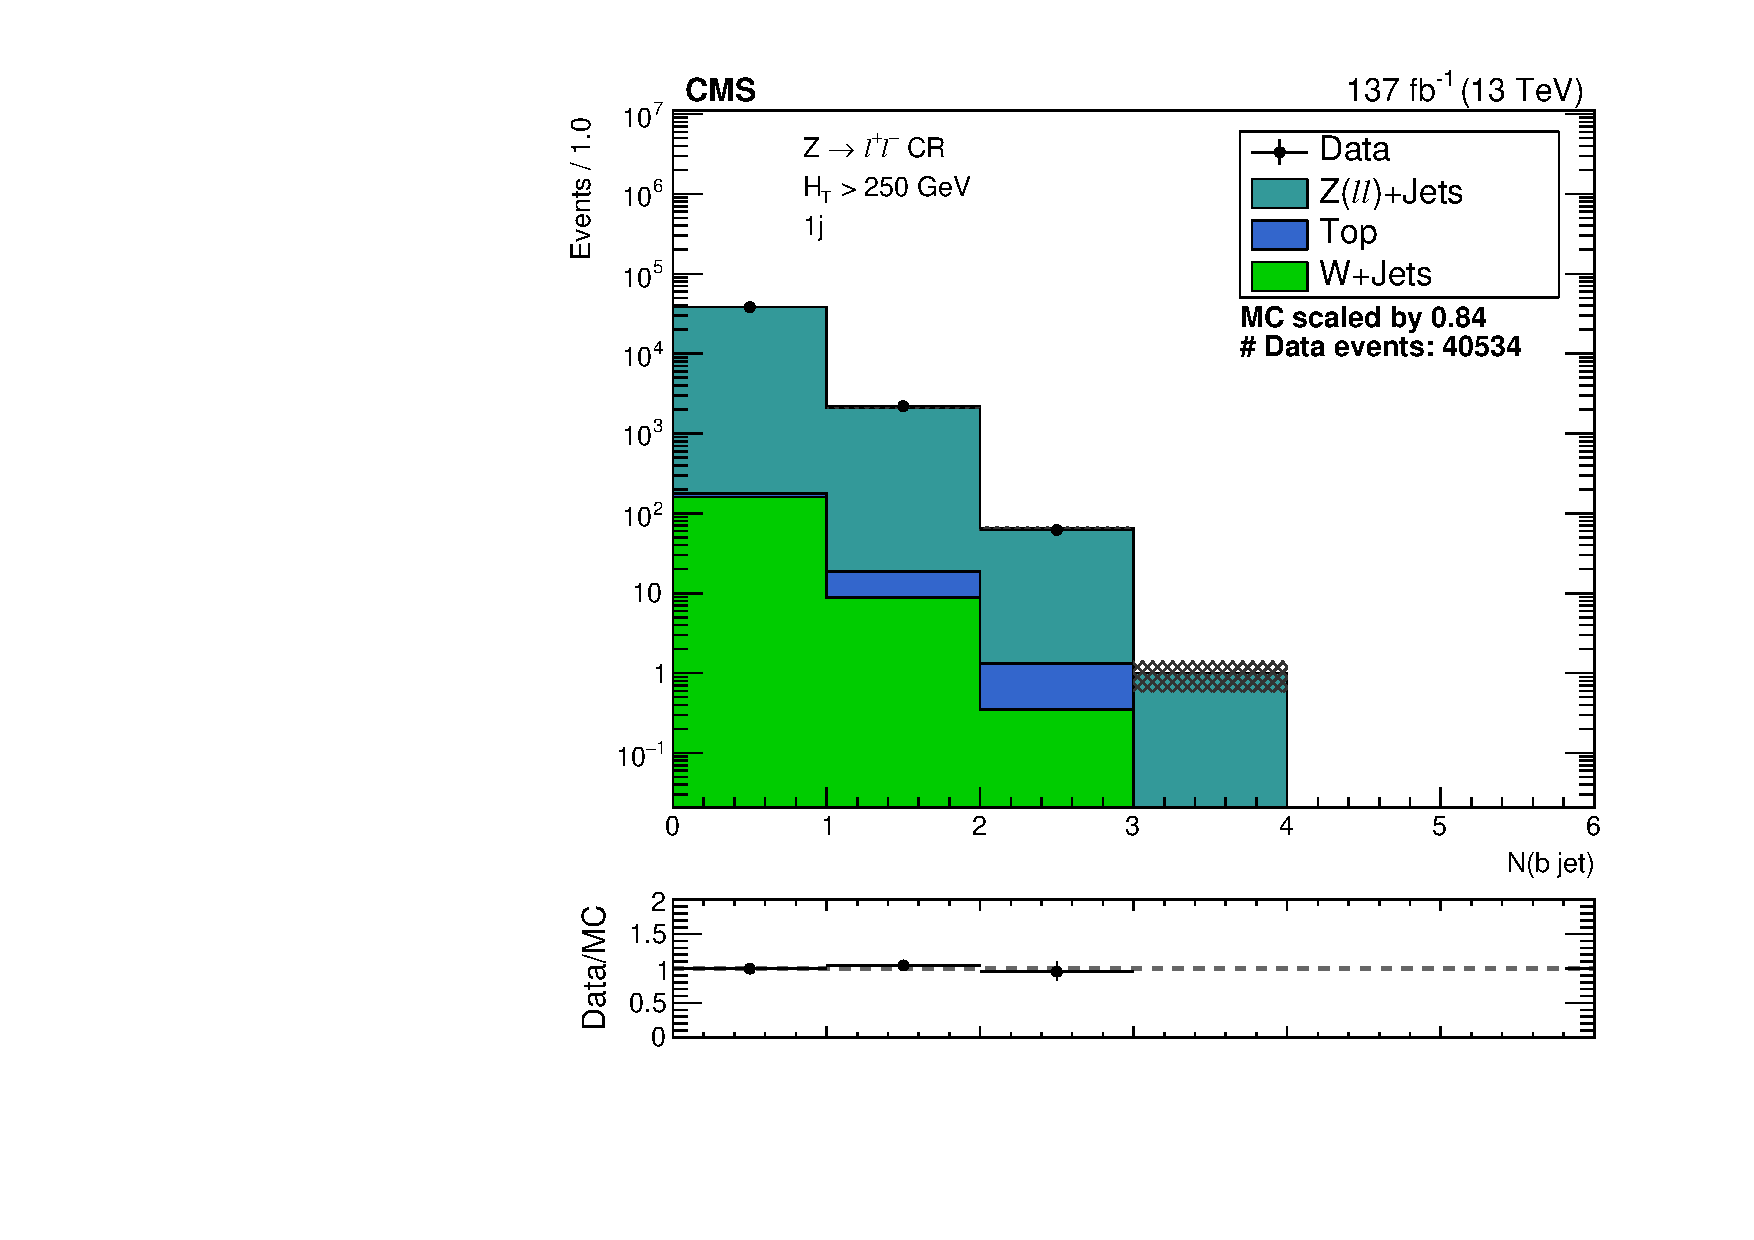
\includegraphics[width=0.47\textwidth]{figs/zinv/crdybaseJ_nBJet20.pdf}
    \caption{Data vs.\ MC comparisons in the baseline \zll control region, for $\Nj\geq2$
      (top two rows), and $\Nj=1$ (bottom row). From left to right, top to bottom, the variables
      plotted are \Ht, \mttwo, \Nj, \Nb, \Ht, and \Nb.
            }
    \label{fig:zll_crplots}
  \end{center}
\end{figure}

The \znunu estimate is first performed in each $(\Ht,\Nj,\Nb)$ topological region, integrated
over \mttwo (for the monojet region, the \Ht dimension is equivalent to $\vSS{p}{T}{\mrm{jet1}}$,
so there is no integration and the estimate is performed in each analysis bin). For all regions
with $\geq$7 jets and $\geq$1 b tag, an inclusive control region with $\geq$7 jets and $\geq$1 b tag
is used, to avoid statistical fluctuations in these regions where \znunu is a subleading background.
Similarly, for regions with 7--9 jets or $\geq$10 jets and 0 b tags, an inclusive control region
with $\geq$7 jets and 0 b tags is used. Since MC is used directly to predict the \Nj and \Nb
shapes here, agreement between data and MC is explicitly checked in these high-\Nj regions.
Fig.~\ref{fig:zll_ge7j} shows data vs.\ MC comparisons of \Nj and \Nb in the $\geq$7 jet region;
sufficient agreement is seen to justify the use of MC in predicting the \Nj and \Nb shapes.
For regions with $\Ht>1500\GeV$, all events with
$\mttwo>200\GeV$ are used in the control region even though the signal region starts at $\mttwo>400\GeV$.
Once the per-topological region estimate is done, a hybrid approach using both data and MC is
used to extrapolate along the \mttwo dimension, as described in Sec.~\ref{sec:zinv_mt2}.

\begin{figure}[ht]
  \begin{center}
    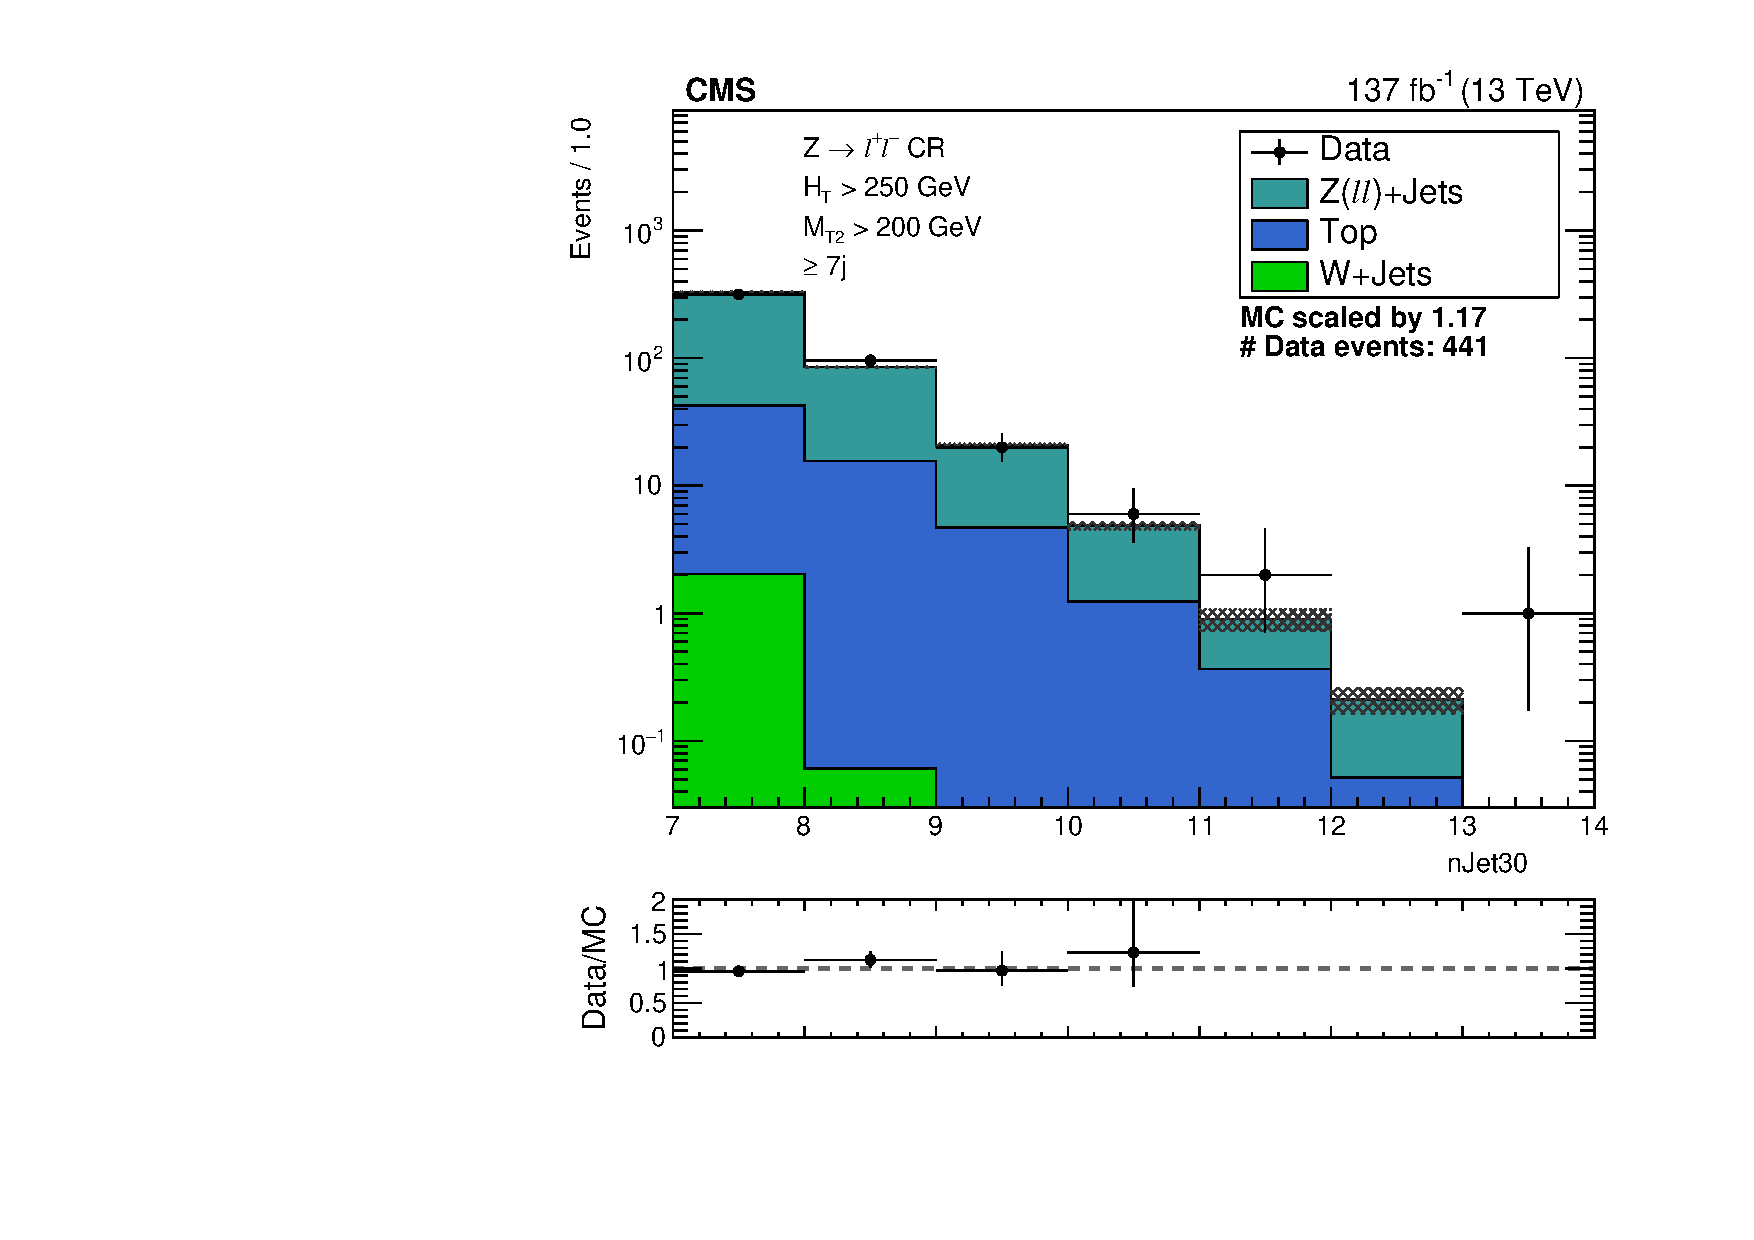
\includegraphics[width=0.48\textwidth]{figs/zinv/crdybase_nJet30_ge7j.pdf}
    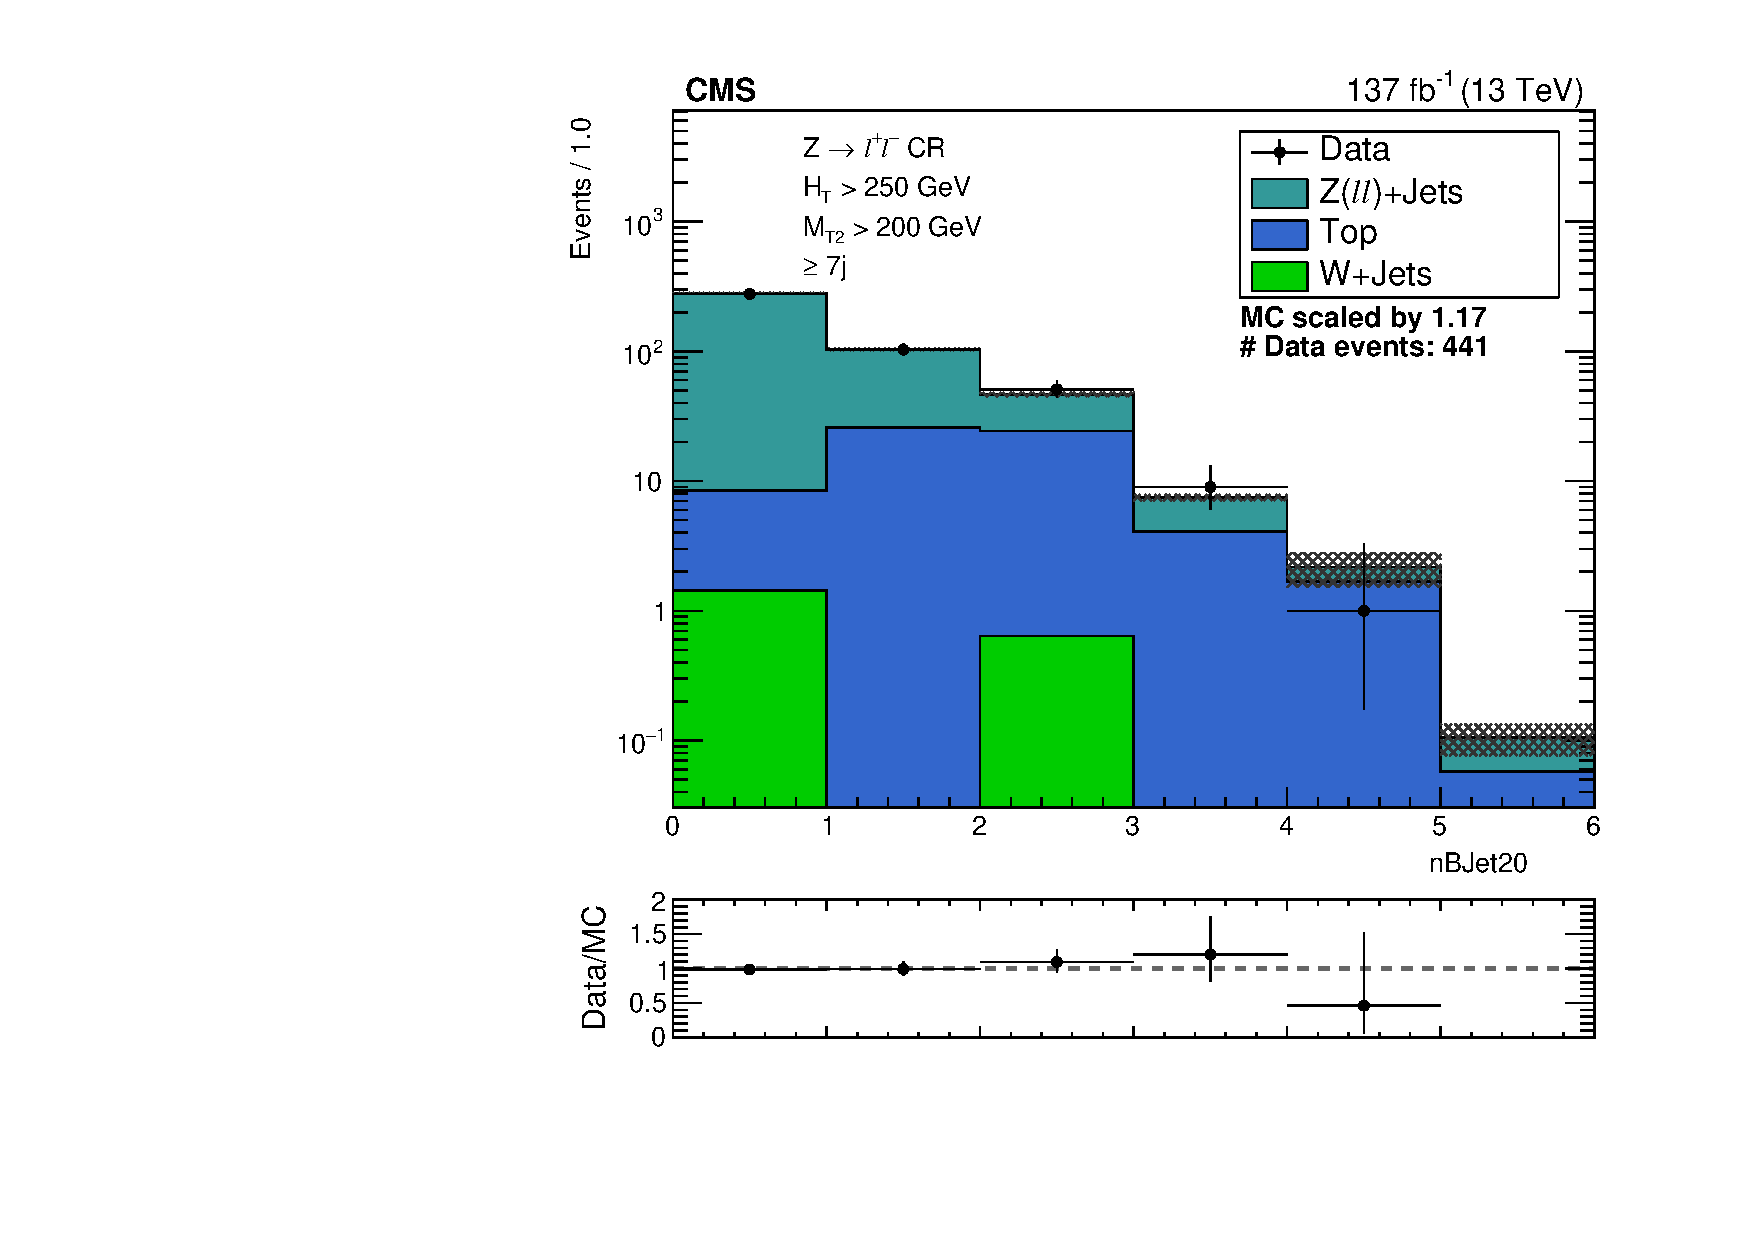
\includegraphics[width=0.48\textwidth]{figs/zinv/crdybase_nBJet20_ge7j.pdf} \\
    \caption{Comparisons of \Nj and \Nb in the $\Nj\geq7$ region. In these high-\Nj regions, 
      shapes of \Nj and \Nb are taken directly from MC as statistics in data are insufficient.
      Monte Carlo is seen to agree well with the observed data in the control region, 
      validating its use to predict signal region yields.
            }
    \label{fig:zll_ge7j}
  \end{center}
\end{figure}


The final estimate in each $(\Ht,\Nj,\Nb,\mttwo)$ signal region can then be summarized as
\be\label{eq:zinv_est}
N_{\znunu}^\mrm{SR} = \left[ N_\mrm{2-lep}^\mrm{CRSF}\; P_{\zll}\; R_\mrm{MC}^{\znunu/\zll} \right]
(\Omega) \times k_\mrm{hybrid}(\mttwo|\Omega),
\ee
where
\begin{itemize}\setlength\itemsep{0mm}
\item $N_\mrm{2-lep}^\mrm{CRSF}$, $P_{\zll}$, and $R_\mrm{MC}^{\znunu/\zll}$ are measured in each topological
region (referred to here as $\Omega\equiv(\Ht,\Nj,\Nb)$), integrated over \mttwo
\item $N_\mrm{2-lep}^\mrm{CRSF}$ is the number of observed events in data in the same-flavor dilepton control region
\item $P_{\zll}$ is the \emph{purity}, or fraction of \zll events in the dilepton control region 
(see Sec.~\ref{sec:dilep_bkgs})
\item $R_\mrm{MC}^{\znunu/\zll}$ is the ratio between \znunu and \zll MC yields in this region
\item $k_\mrm{hybrid}(\mttwo|\Omega)$ is a normalized template used to distribute events as a function
of \mttwo in each topological region (see Sec.~\ref{sec:zinv_mt2}).
\end{itemize}

\subsection{\zll purity in the dilepton control region}
\label{sec:dilep_bkgs}
While \zll is the process of interest in the dilepton control region, other SM processes can
produce similar same-flavor dilepton signatures. Most prominent is \ttbar production, but other
processes contribute in more minor ways, such as $t\bar{t}V$, diboson, and \wjets (with a fake
lepton) production.

Certain kinematic cuts placed in the dilepton control region ensure that the contributions
from these other processes are as small as possible. The $|m_{\ell\ell}-m_Z|<20\GeV$ cut requires
that the dilepton mass is consistent with $Z$ boson decay. Furthermore, the $\pt(\ell\ell)>200\GeV$ cut
selects events in which the leptons are the primary souce of \ptmiss in the event (once their \vSS{p}{T}{}
vectors are added to the \vMet). When this is the case, the $\ptmiss>250\GeV$ cut means that
$\pt(\ell\ell)$ must be large. If, however, there are contributions to the \ptmiss from actual
invisible particles (such as the neutrinos present in all of the secondary production modes listed above),
$\pt(\ell\ell)$ is generally smaller. This is illustrated in Fig.~\ref{fig:zllpt}, which shows a distribution
of $\pt(\ell\ell)$ in the baseline dilepton control region (with the $m_{\ell\ell}$ cut inverted for
$\pt(\ell\ell)<200\GeV$). We see that the $\pt(\ell\ell)>200\GeV$ region is almost entirely from \zll events,
and the $\pt(\ell\ell)<200\GeV$ region comes predominantly from top (\ttbar and $t\bar{t}V$) processes.

Despite the attempts made to purify the control region with \zll events, there is nevertheless some contamination
from non-$Z$ processes. To estimate and subtract off this contamination, we make use of the fact that
all of the secondary processes are flavor-symmetric, in that they produce opposite-flavor ($e\mu$) events
at the same rate as same-flavor ($ee$ or $\mu\mu$) events. Hence, we can measure their rate in an 
opposite-flavor (OF) control region (same cuts as the nominal same-flavor (SF) dilepton control region, but 
requiring one $e$ and one $\mu$), and then convert this to an estimated same-flavor rate by 
multiplying by a transfer factor $R^\mrm{SF/OF}$.

\begin{figure}[ht]
  \begin{center}
    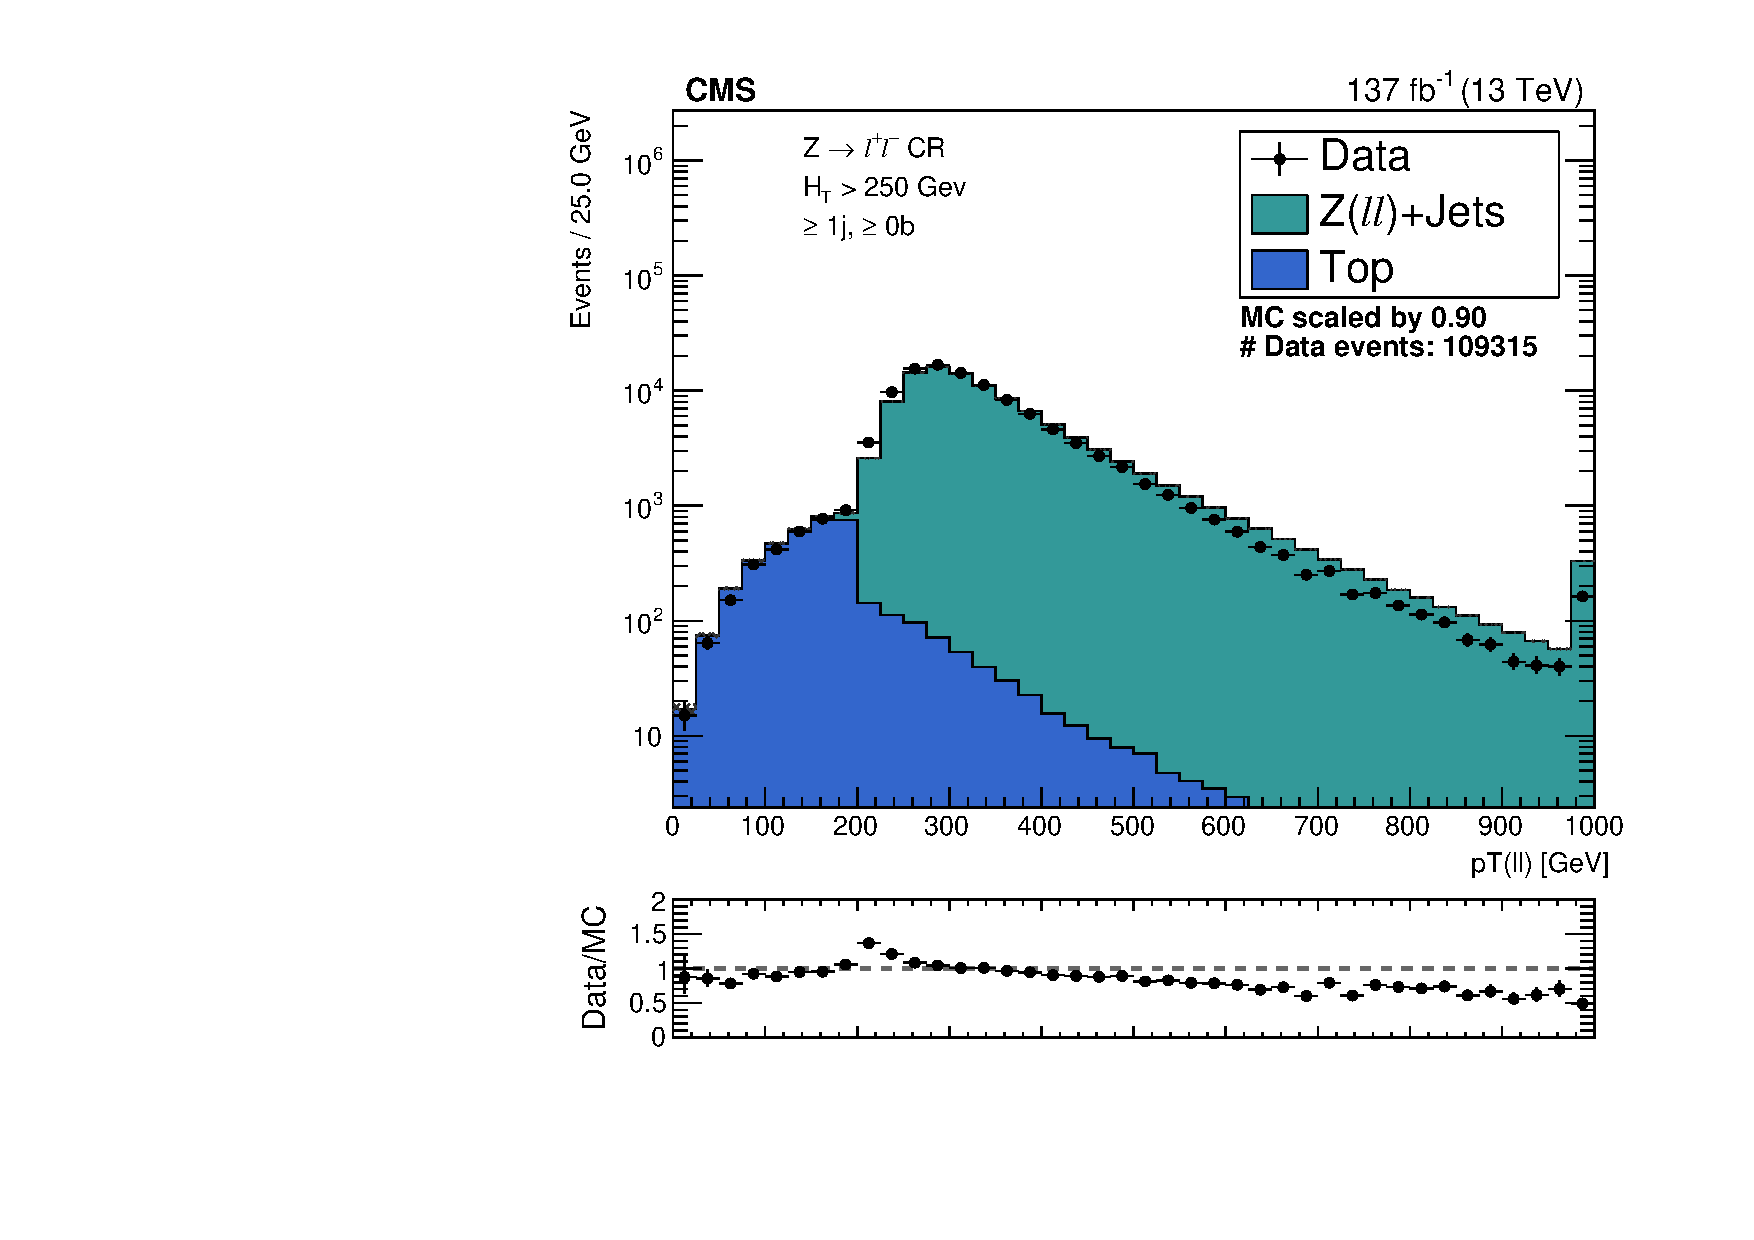
\includegraphics[width=0.55\textwidth]{figs/zinv/crdybase_zllpt.pdf}
    \caption{$\pt(\ell\ell)$ in the baseline dilepton control region, with the exception
      of the $|m_{\ell\ell}-m_Z|<20\GeV$ cut which is inverted for the $\pt(\ell\ell)<200\GeV$
      portion of the plot. We see that the $m_{\ell\ell}$ and $\pt(\ell\ell)$ requirements ensure
      that the control region is predominantly from \zll, and inverting these requirements produces
      a region enriched in top processes (used to measure $R^\mrm{SF/OF}$).
            }
    \label{fig:zllpt}
  \end{center}
\end{figure}

While this SF/OF ratio is in theory equal to 1 at the production level (since branching fractions to electrons
and muons are the same), different reconstruction efficiencies for electrons and muons cause it to deviate 
from 1 at the reconstructed level. We measure this ratio in data in a top-enriched dilepton control region,
which is the same as the baseline dilepton control region but with $|m_{\ell\ell}-m_Z|>20\GeV$ and
$\pt(\ell\ell)<200\GeV$ (the portion of Fig.~\ref{fig:zllpt} with $\pt(\ell\ell)$ below 200 GeV).
The measurement is done inclusively in all analysis variables, to get a single number that is applied 
to every topological region. The measured ratio is plotted as a function of the analysis variables to
ensure that it is actually constant, and a systematic uncertainty on $R^\mrm{SF/OF}$ is assessed to
cover for any observed variation.

\begin{figure}[ht]
  \begin{center}
    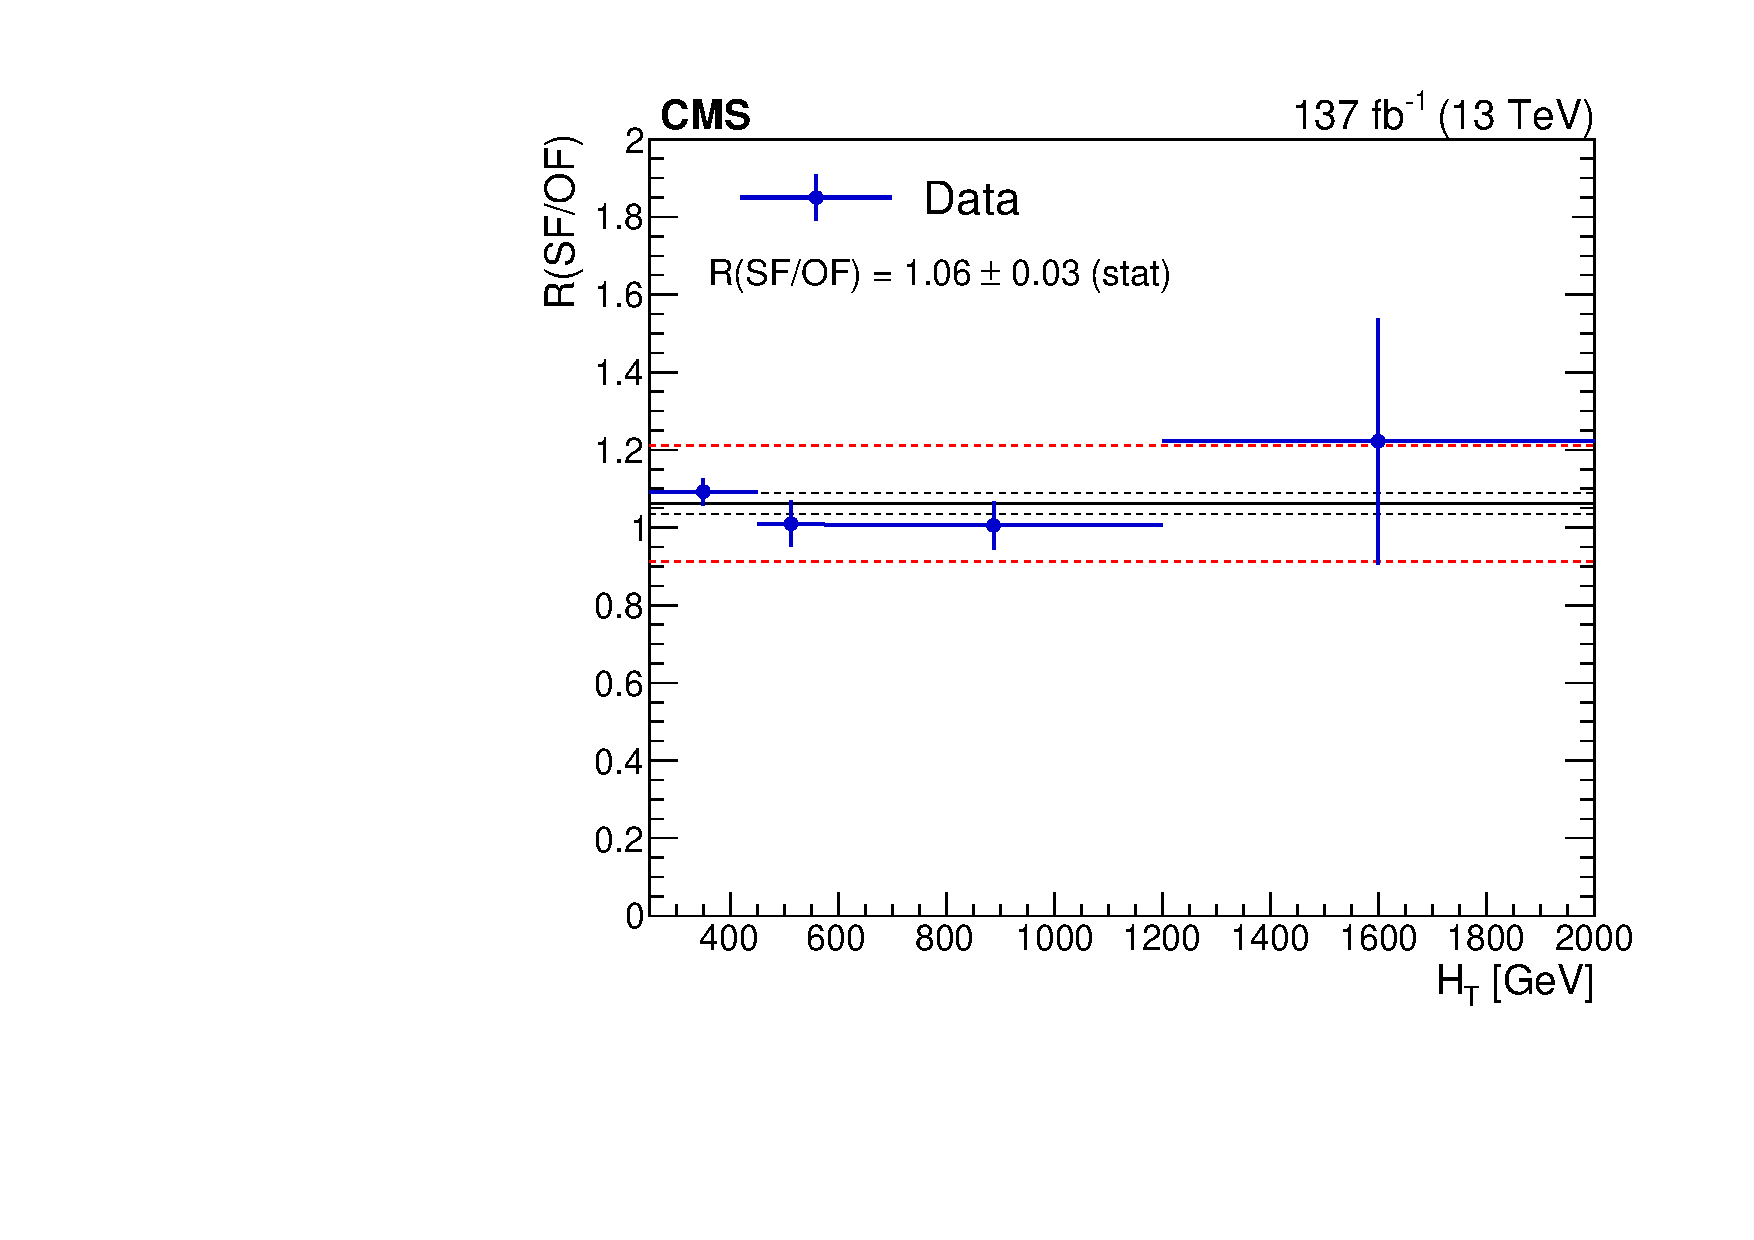
\includegraphics[width=0.48\textwidth]{figs/zinv/rsfof_ht.pdf}
    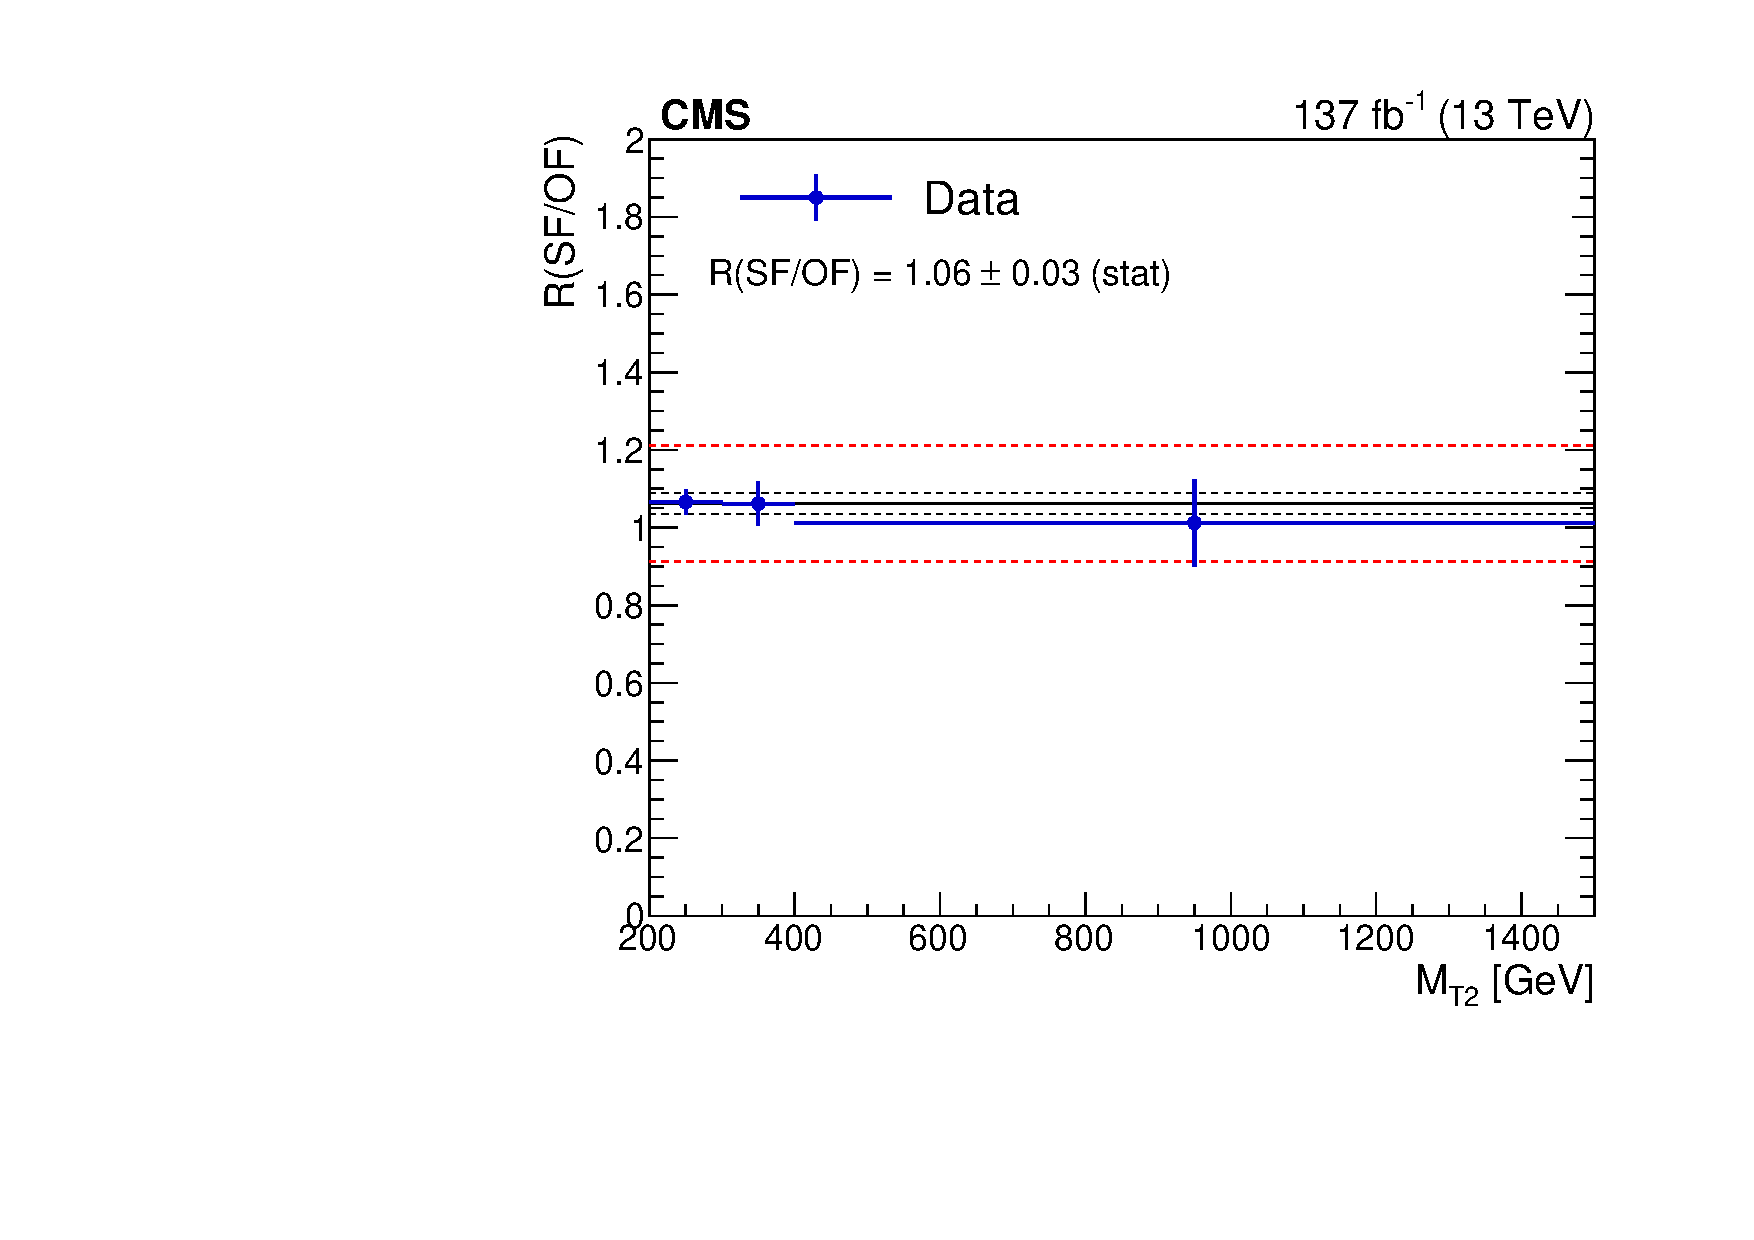
\includegraphics[width=0.48\textwidth]{figs/zinv/rsfof_mt2.pdf} \\
    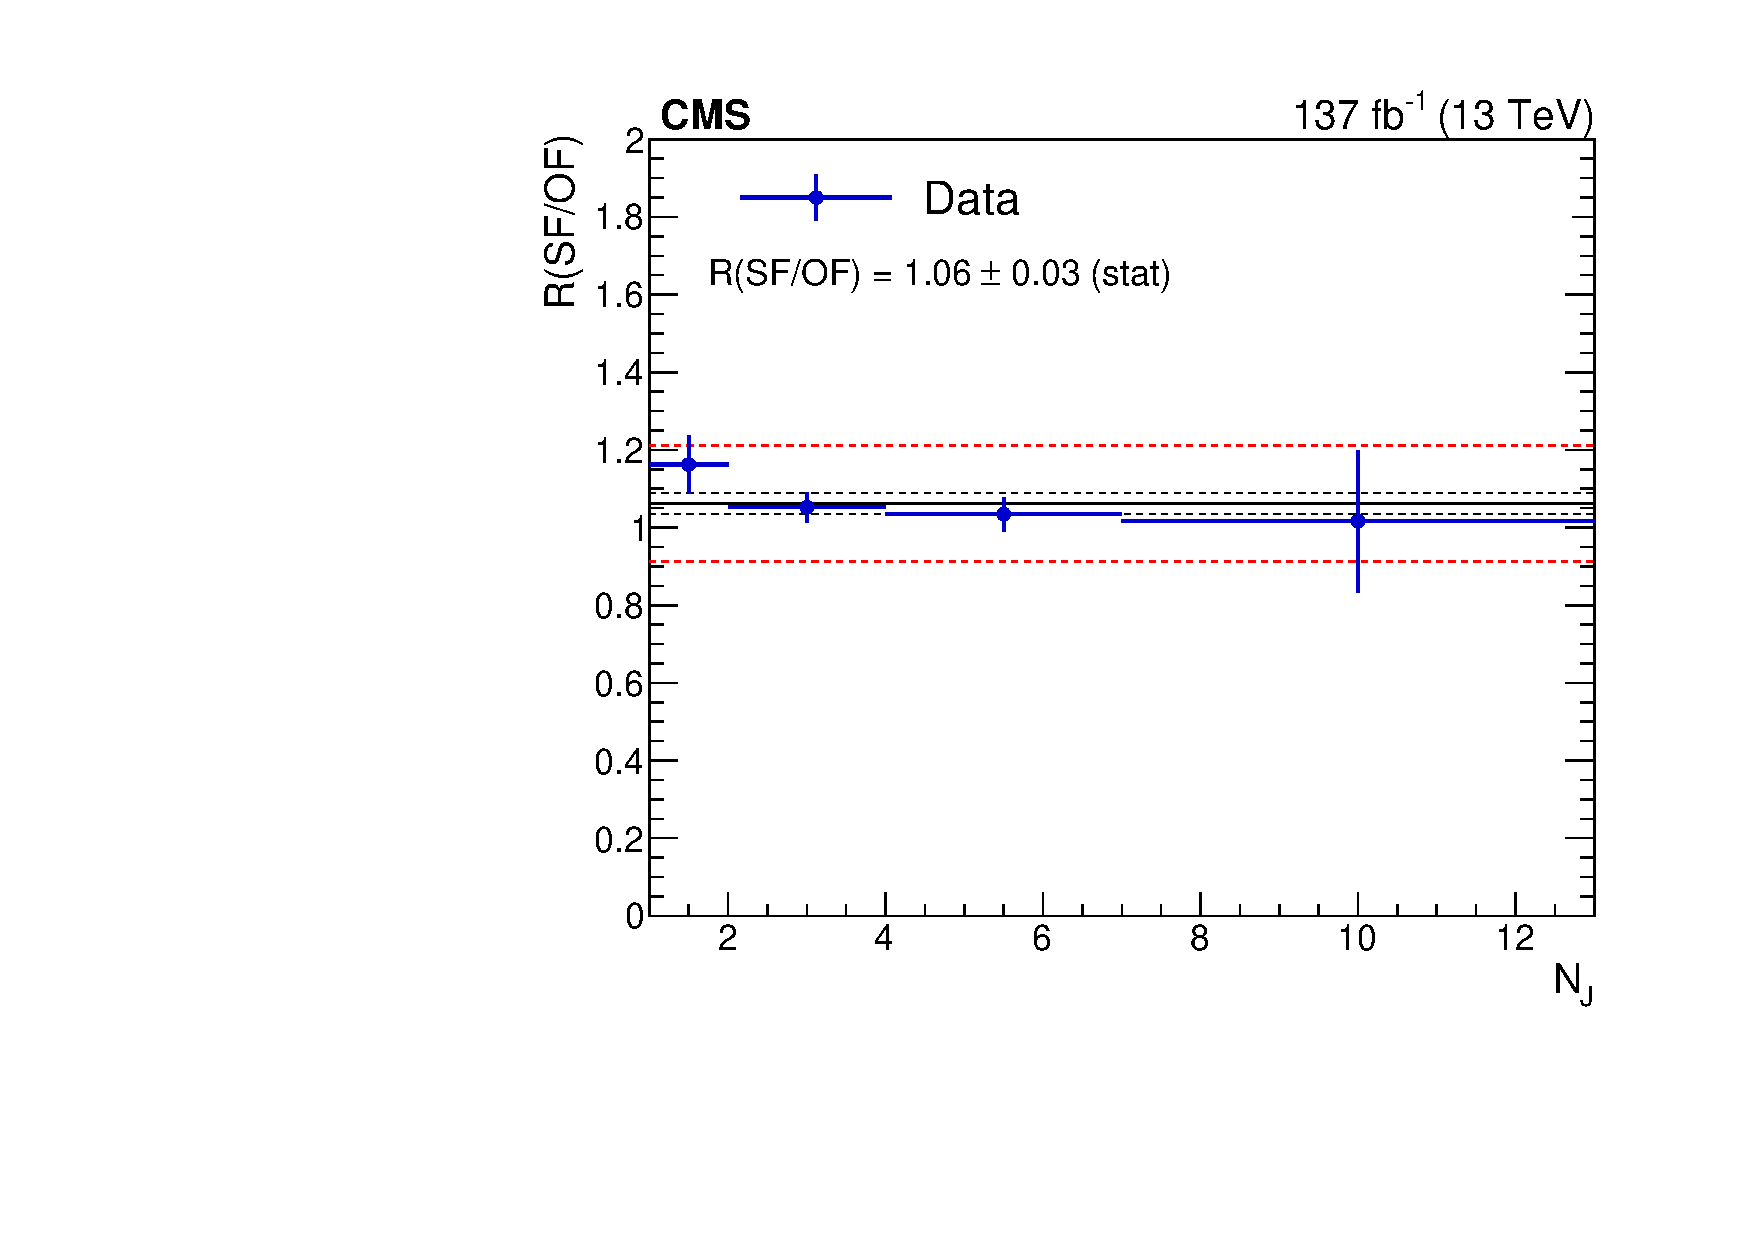
\includegraphics[width=0.48\textwidth]{figs/zinv/rsfof_nJet30.pdf}
    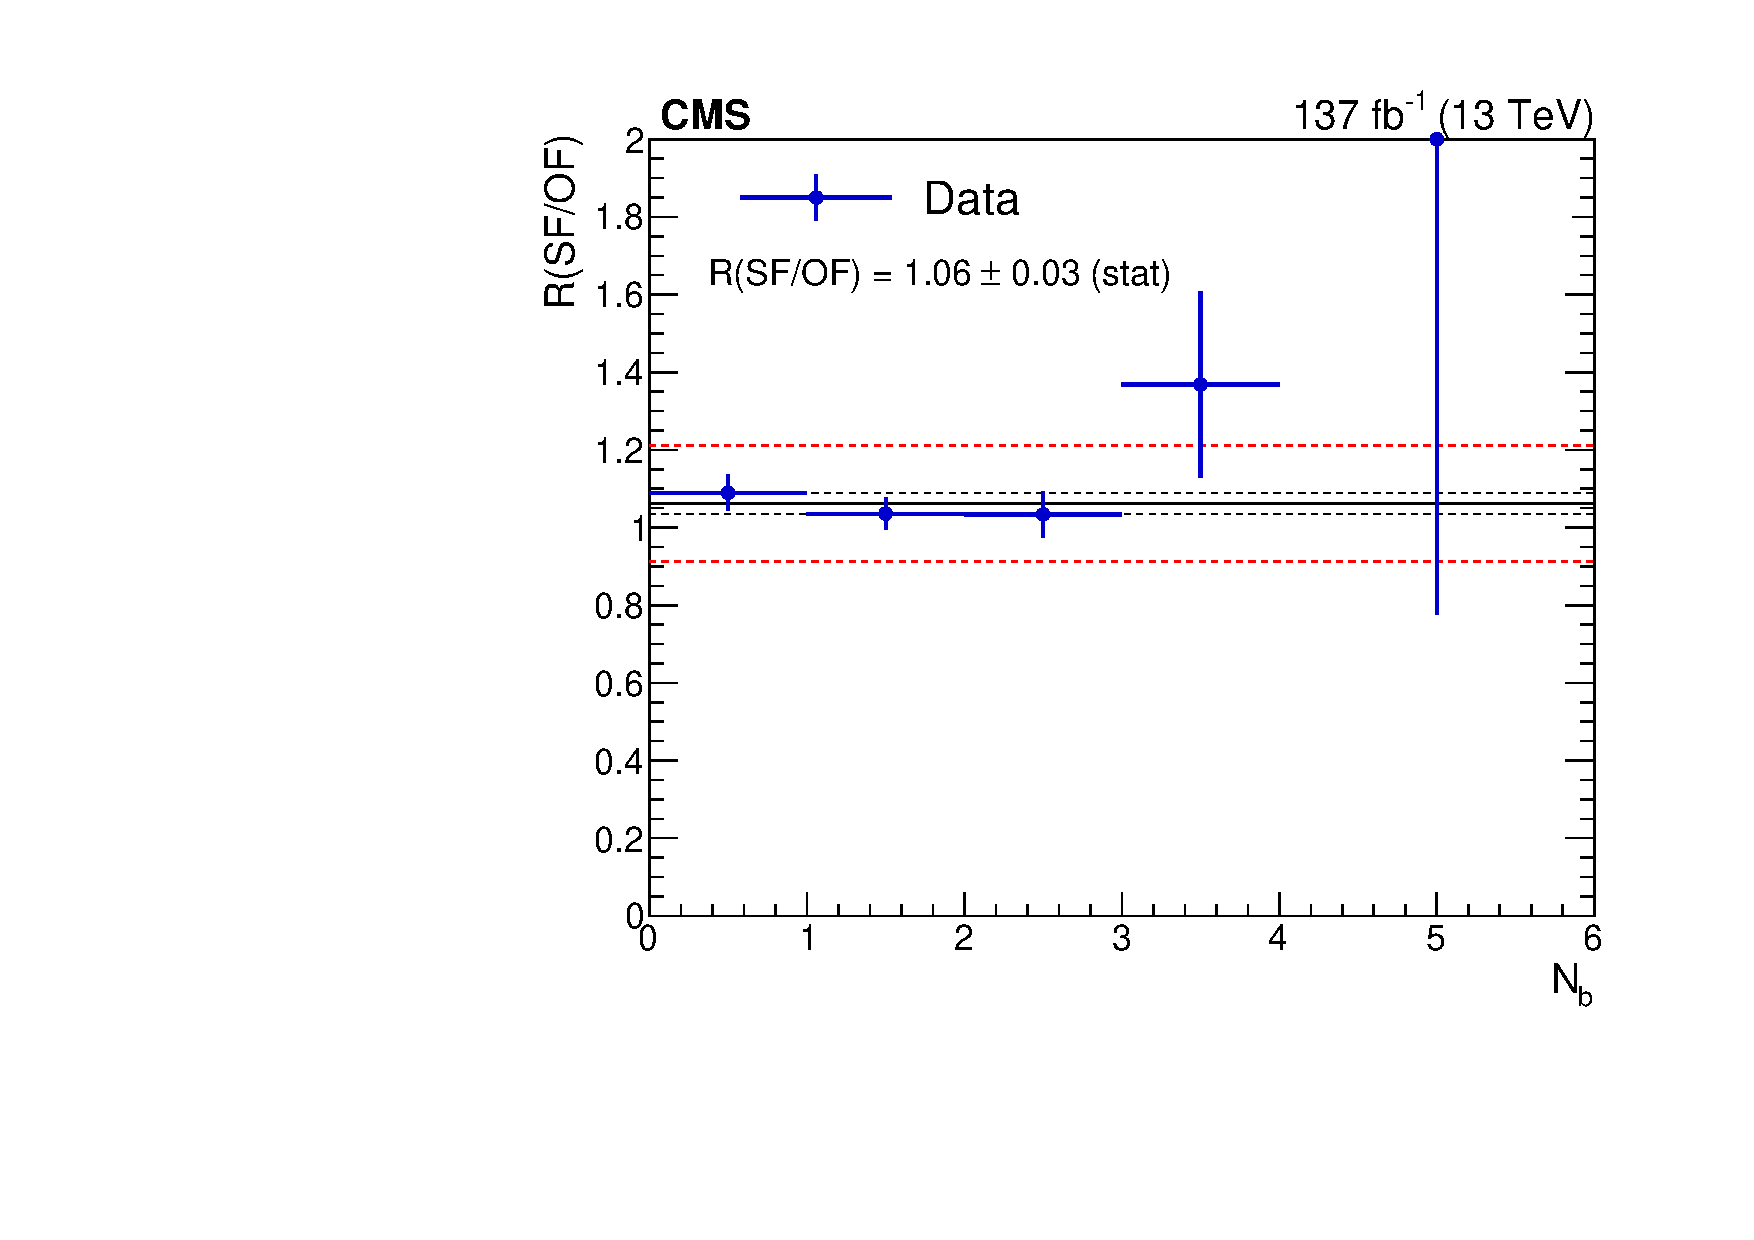
\includegraphics[width=0.48\textwidth]{figs/zinv/rsfof_nBJet20.pdf}
    \caption{Measured $R^\mrm{SF/OF}$ as a function of \Ht, \mttwo, \Nj, and \Nb.
      The black lines show the measured value of $1.06\pm0.03$. The dotted red lines
      show the 15\% systematic uncertainty assessed to cover for any kinematic variation
      in the ratio.
            }
    \label{fig:rsfof}
  \end{center}
\end{figure}

This is illustrated in Fig.~\ref{fig:rsfof}, in which $R^\mrm{SF/OF}$ as measured in data is plotted
as a function of \Ht, \mttwo, \Nj, and \Nb. The ratio is measured to be $1.06\pm0.03$, and is seen to 
be approximately independent of the kinematic variables. To cover for the small observed variation, 
a systematic uncertainty of 0.15 is placed on $R^\mrm{SF/OF}$ and propagated to the final estimate.

Once $R^\mrm{SF/OF}$ is measured, we can compute the purity $P_{\zll}$ used in Eq.~\ref{eq:zinv_est} 
(measured independently in each topological region as) as
\be
P_{\zll} = 1 - R^\mrm{SF/OF} N_\mrm{2-lep}^\mrm{CROF} / N_\mrm{2-lep}^\mrm{CRSF},
\ee
where $N_\mrm{2-lep}^\mrm{CROF}$ is the number of observed events in data in the opposite-flavor
dilepton control region.



\section{\texorpdfstring{\mttwo}{MT2} extrapolation}
\label{sec:zinv_mt2}

To project the per-topological region estimate described in the previous section along the \mttwo dimension, we use
a ``hybrid'' \mttwo template derived using both data and MC ($k_\mrm{hybrid}(\mttwo|\Omega)$ in Eq.~\ref{eq:zinv_est}).

In every \Ht region, the \mttwo shape for both \znunu and \zll MC events is observed to be independent of \Nb.
An example of this is shown in Fig.~\ref{fig:zinv_nbshape}, for the medium \Ht region. Furthermore,
in the extreme \Ht region ($[1500,\infty]\GeV$), the \mttwo shape is observed to also be independent of \Nj
up to \mttwo values of about 1\TeV.

Thus, we build \mttwo shape templates from data and MC in each $(\Ht,\Nj)$ bin for regions
with $\Ht<1500\GeV$, integrating over \Nb, while one single hybrid template is built for the
extreme $\Ht>1500\GeV$ region, integrating also over \Nj. The one exception is for regions with
exactly 2 or 2--6 jets and $\geq$3 b tags. To avoid sculpting the \Nj distribution by requiring
$\Nb\geq3$, we use regions with $\Nj\geq3$ to obtain \mttwo shape templates in these regoins.

\begin{figure}[ht]
  \begin{center}
    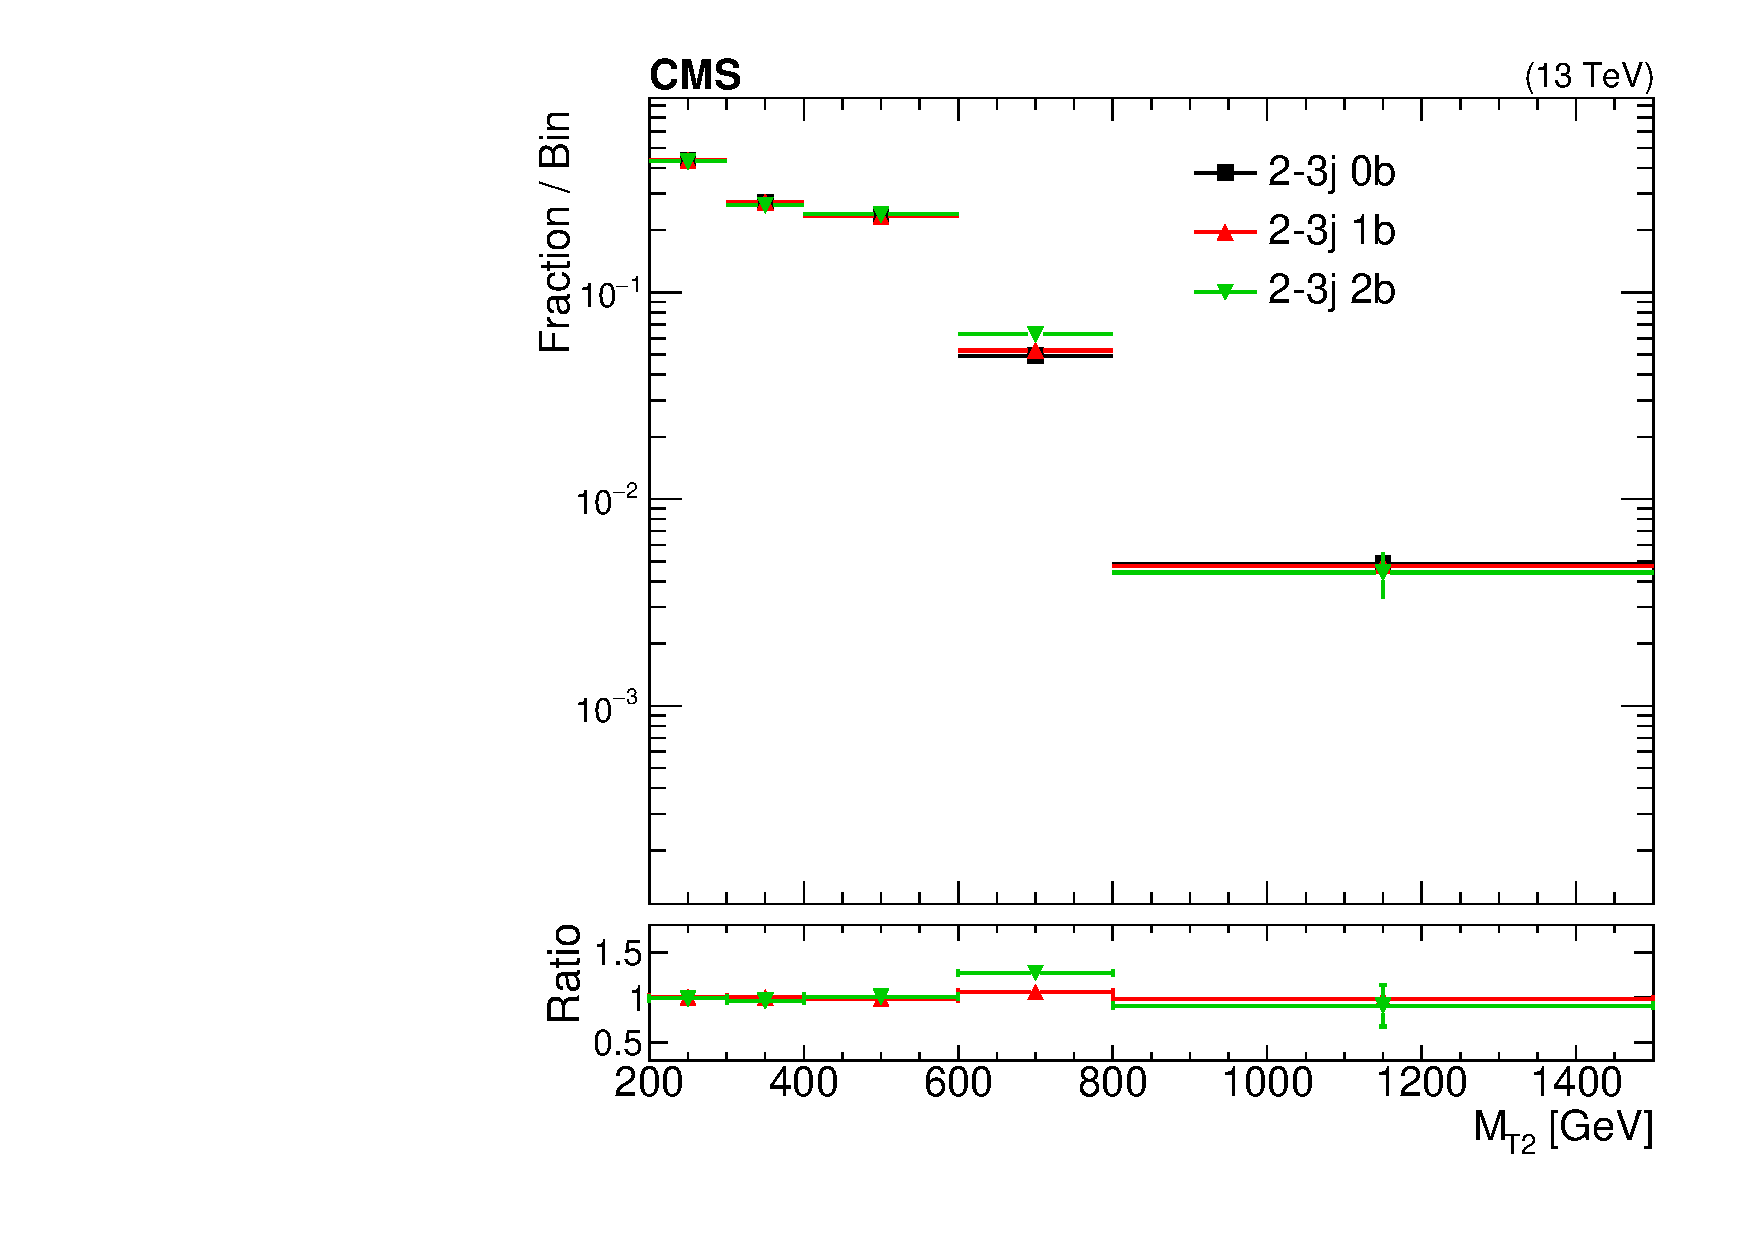
\includegraphics[width=0.24\textwidth]{figs/zinv/MT2vsNB_1M.pdf}
    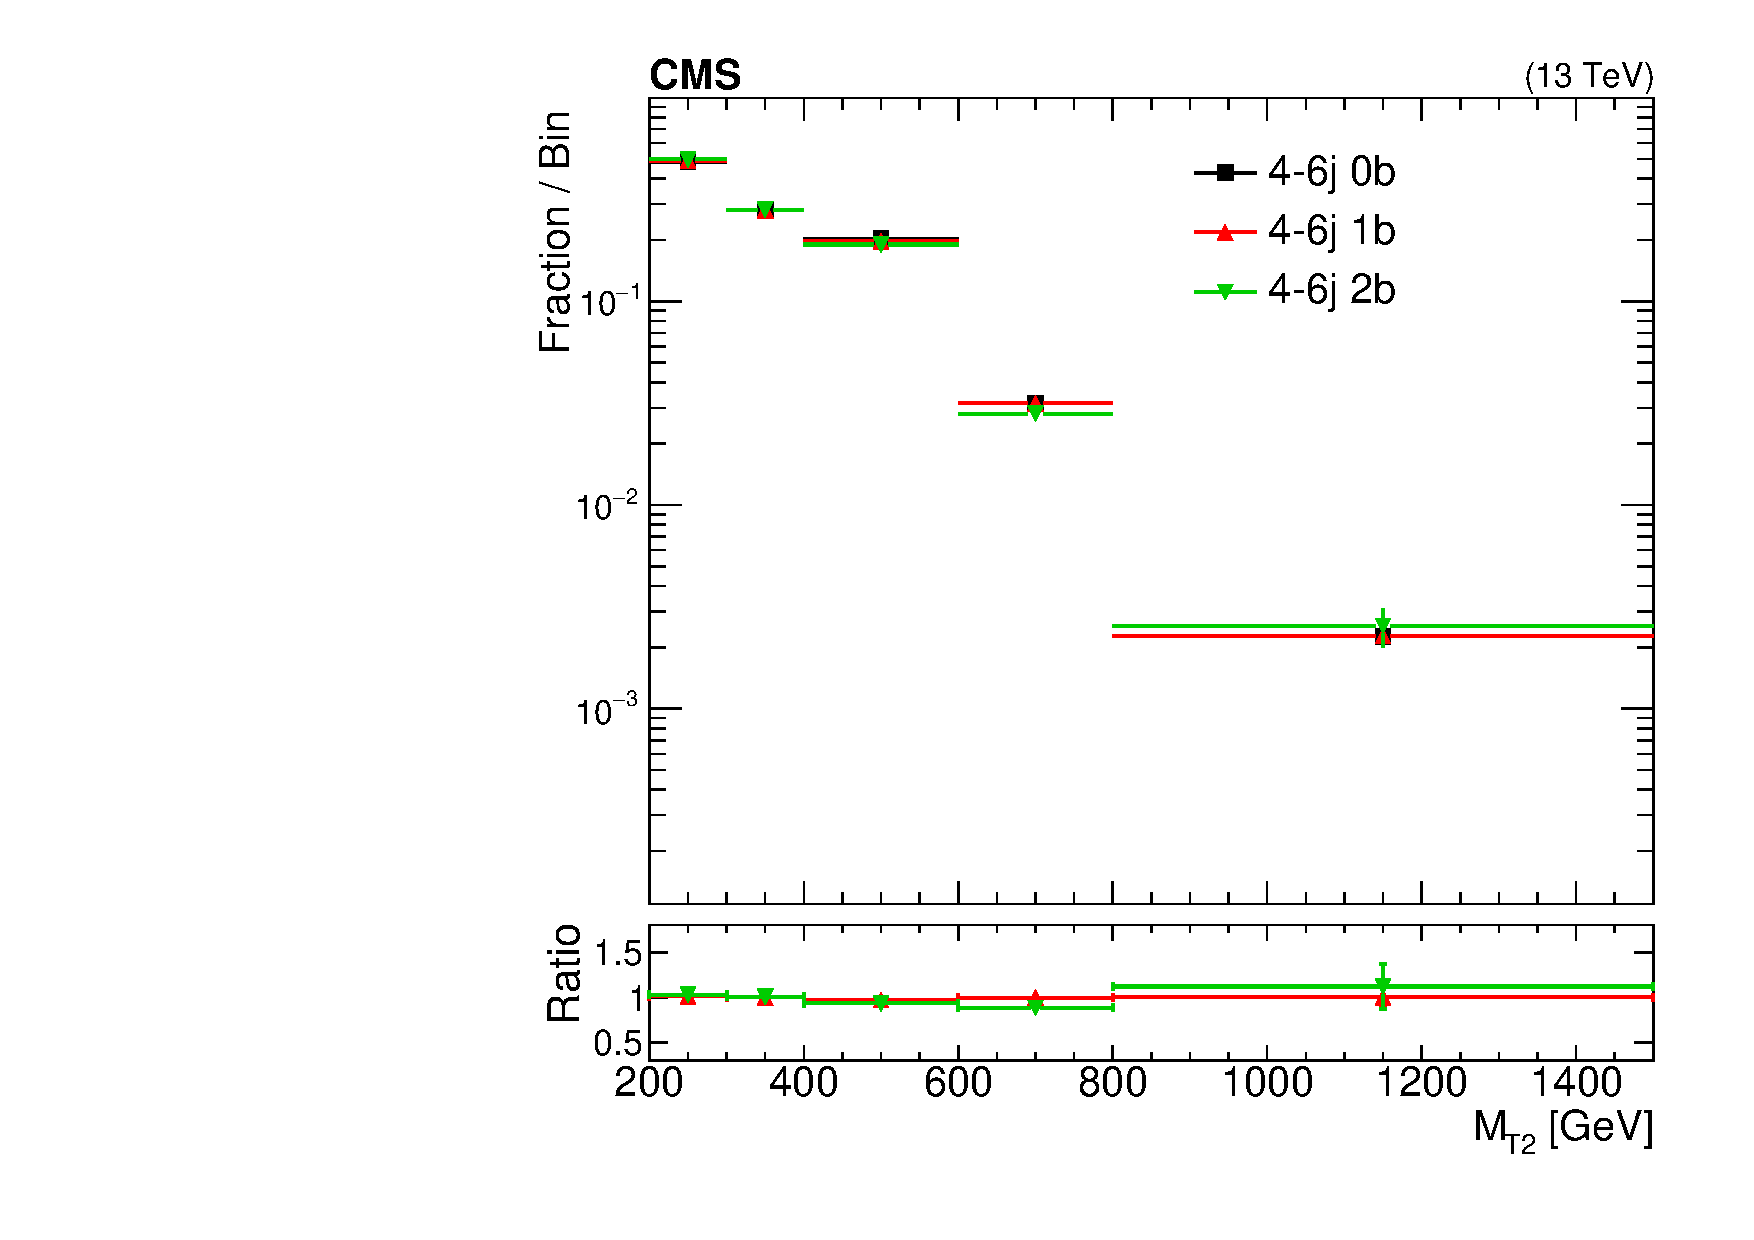
\includegraphics[width=0.24\textwidth]{figs/zinv/MT2vsNB_4M.pdf}
    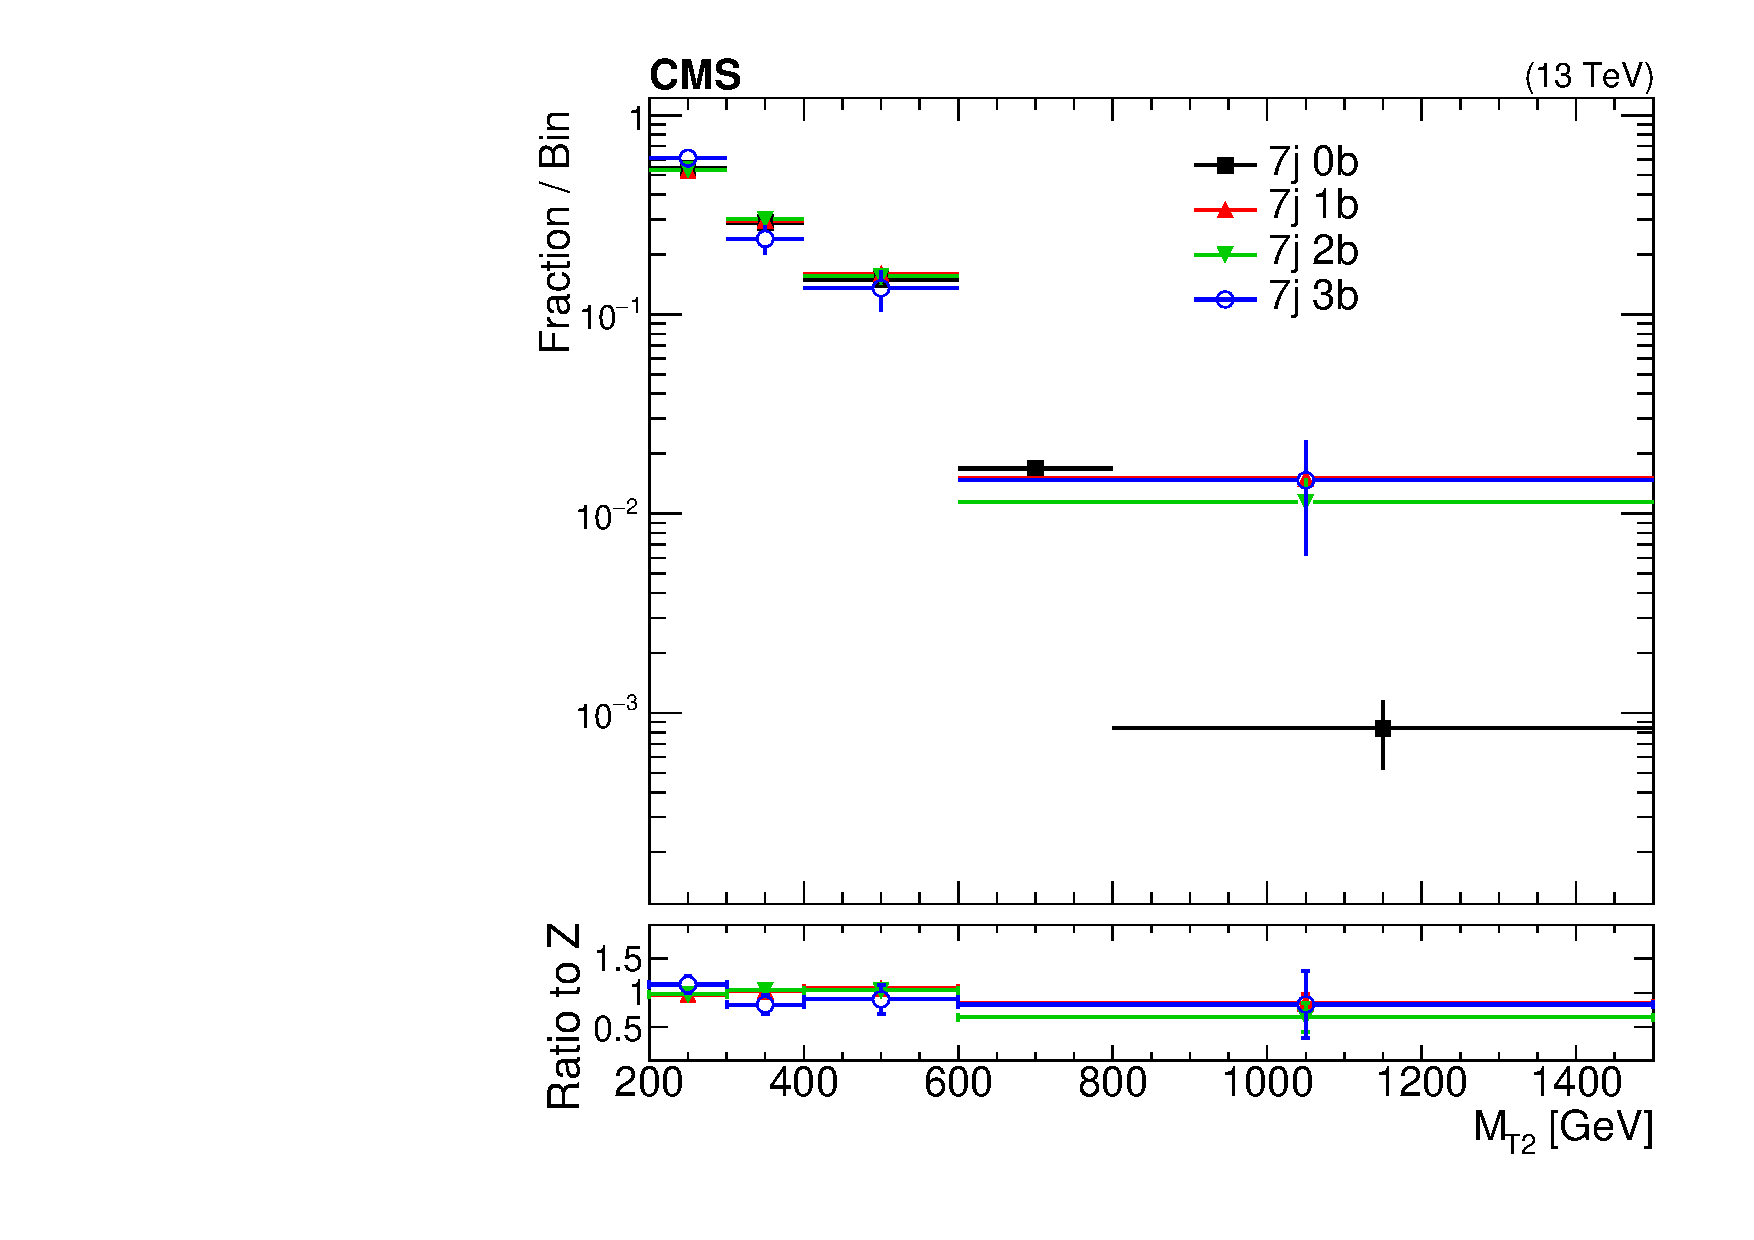
\includegraphics[width=0.24\textwidth]{figs/zinv/MT2vsNB_7M.pdf}
    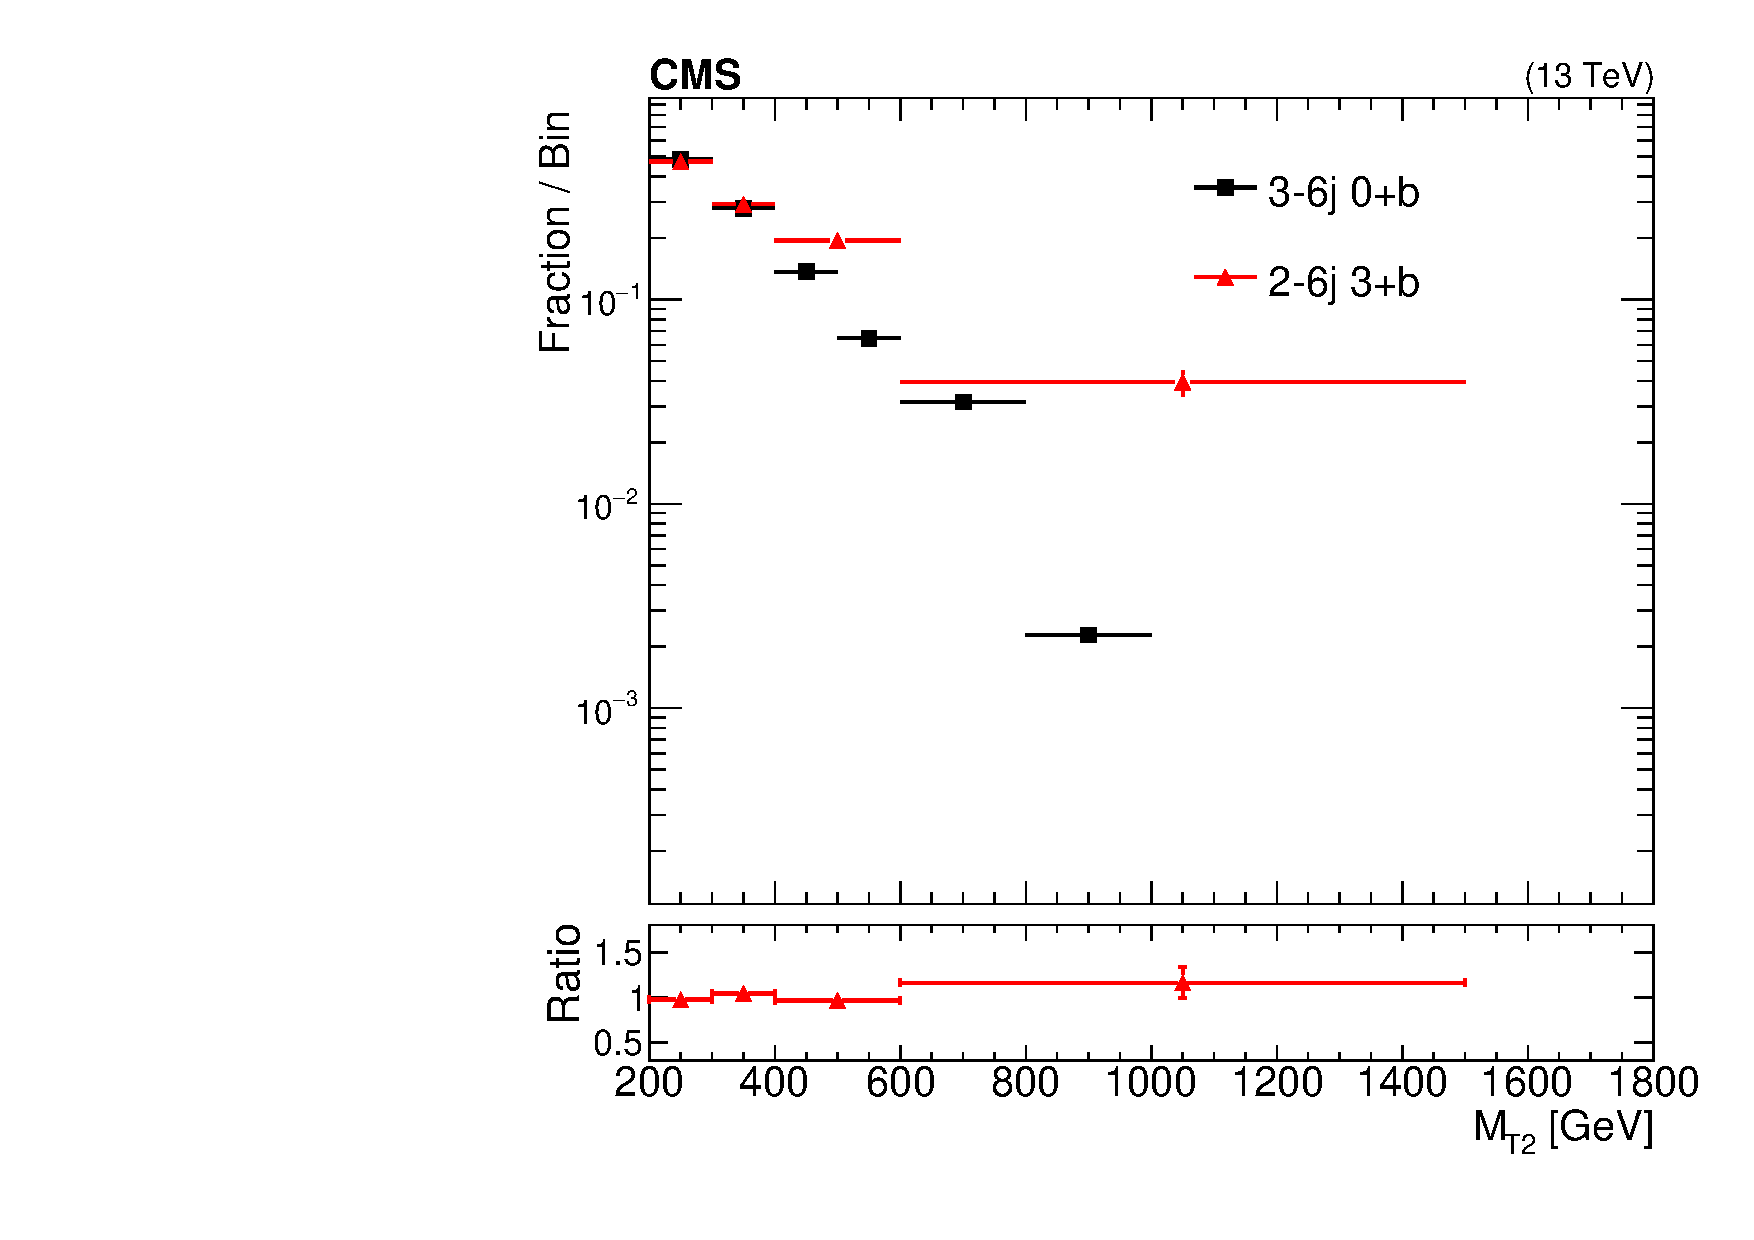
\includegraphics[width=0.24\textwidth]{figs/zinv/MT2vsNB_26M.pdf} \\
    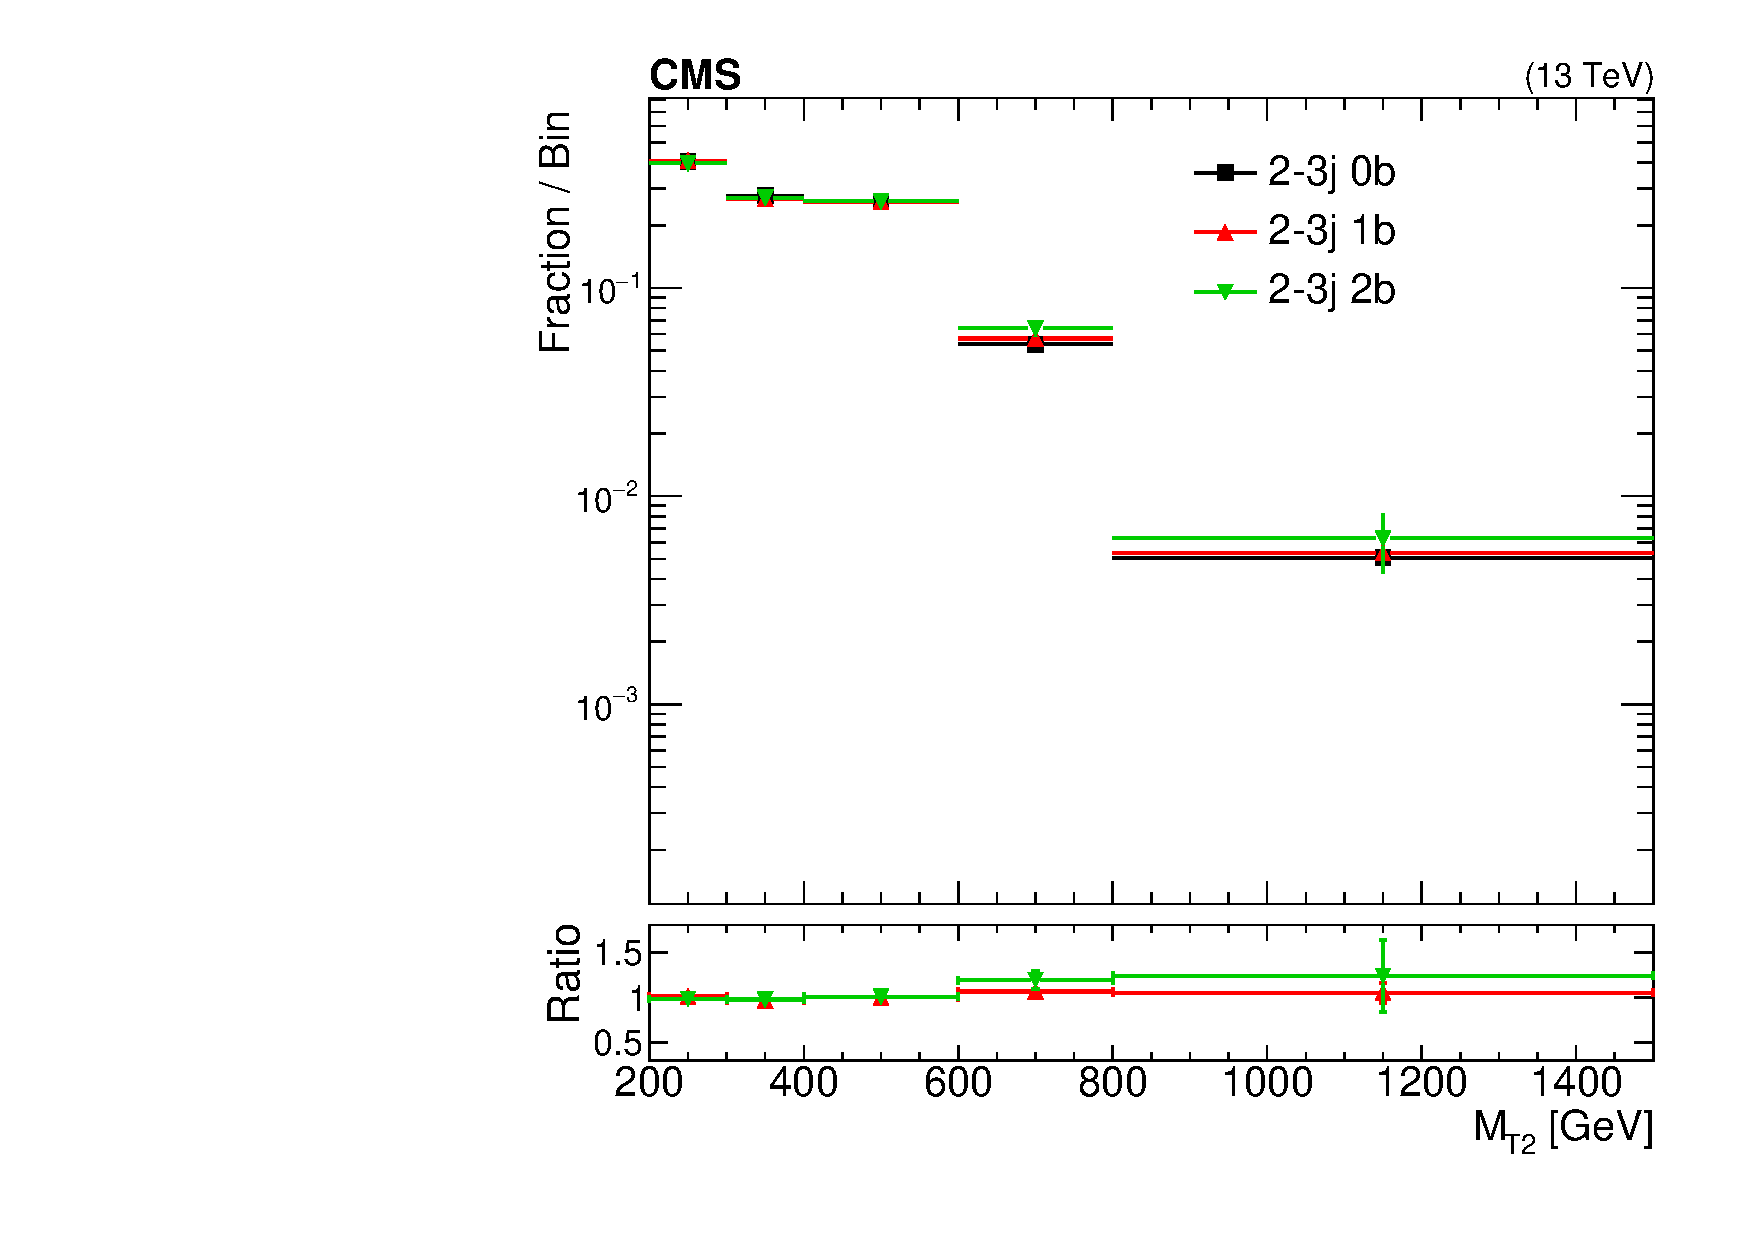
\includegraphics[width=0.24\textwidth]{figs/zinv/MT2vsNB_1MDY.pdf}
    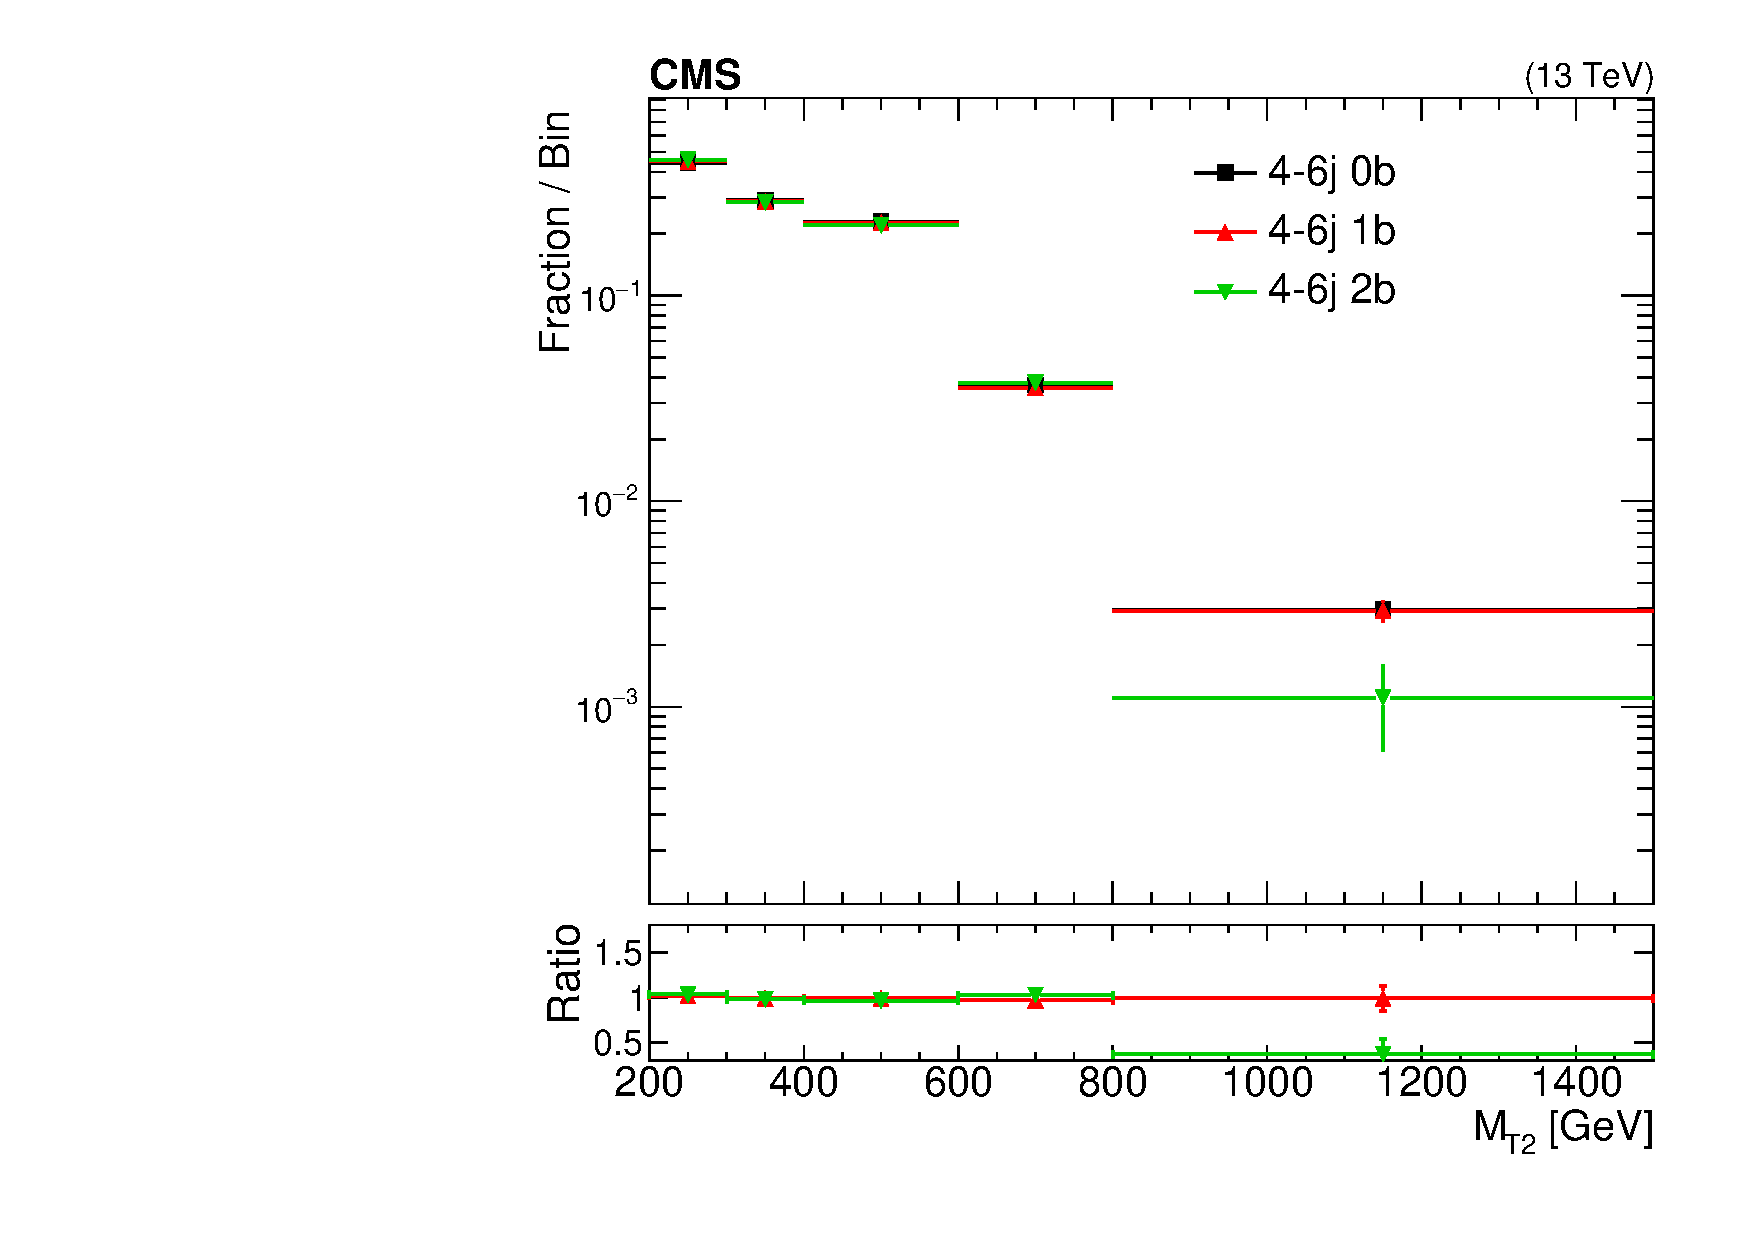
\includegraphics[width=0.24\textwidth]{figs/zinv/MT2vsNB_4MDY.pdf}
    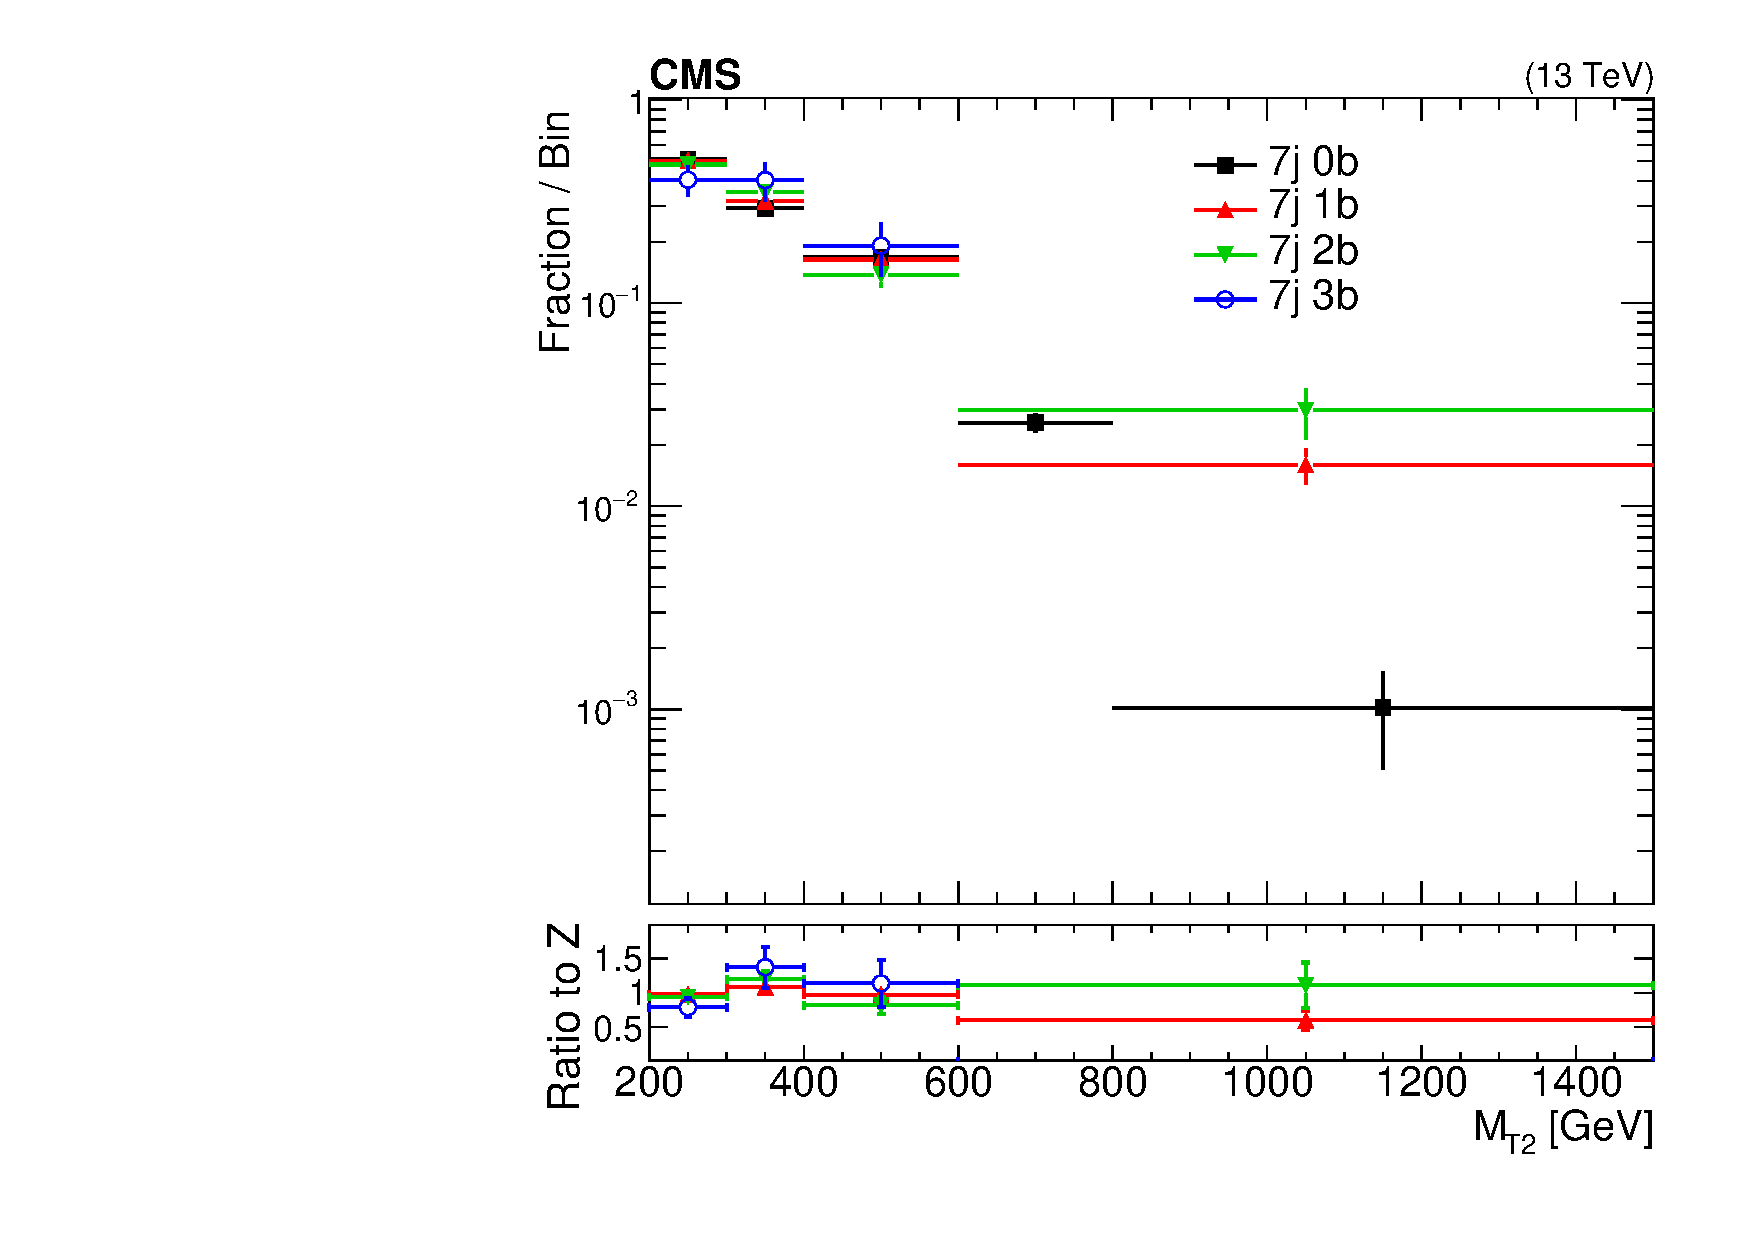
\includegraphics[width=0.24\textwidth]{figs/zinv/MT2vsNB_7MDY.pdf}
    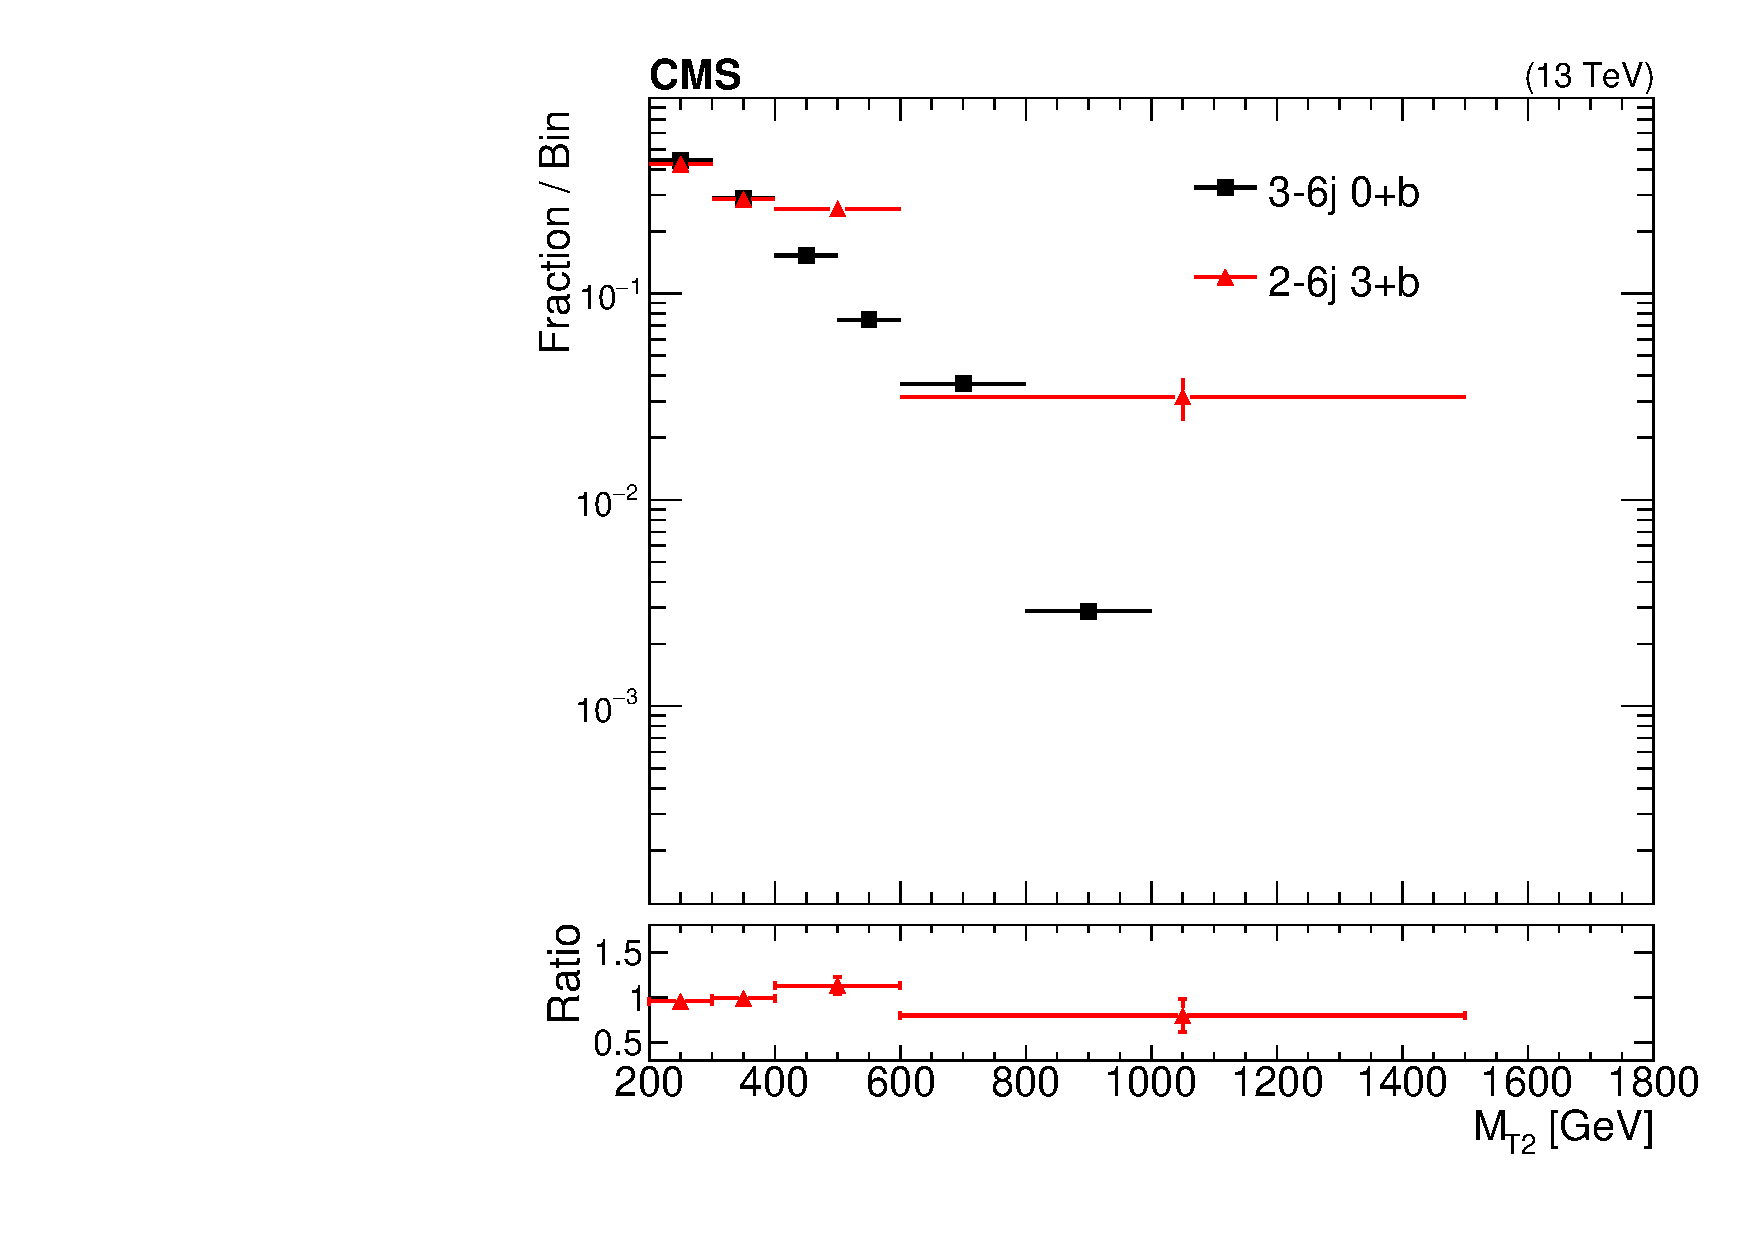
\includegraphics[width=0.24\textwidth]{figs/zinv/MT2vsNB_26MDY.pdf} \\
    \caption{Example \mttwo distributions in various bins of \Nj and \Nb in the
      \Ht region $[575,1000]\GeV$, for \zll (top) and \znunu (bottom) MC.
      We see that the \mttwo shape is independent of \Nb in all \Nj regions.
            }
    \label{fig:zinv_nbshape}
  \end{center}
\end{figure}

Starting from the highest \mttwo bin in each topological region in the dilepton control region,
we merge bins until the sum of expected yields in the merged bins is at least 50 events, 
as predicted by MC for the full integrated luminosity of \Lint.
For the lower non-merged \mttwo bins, which have larger statistics, the \mttwo shapes are built
directly from \zll data, corrected by the \znunu/\zll MC ratio in order to account
for lepton reconstruction effects. The \znunu MC \mttwo shape is instead used to distribute
events across the merged \mttwo bins, after renormalizing the MC to the total data yield in
the same bins. For the $\Ht>1500\GeV$ region, we use \Nj-binned \znunu MC shapes for 
the extrapolation, to avoid the mild \Nj dependence observed at high \mttwo.

For the lower \mttwo bins, where the \mttwo shapes are built directly from \zll data, an
uncertainty corresponding to the statistical uncertainty in data in each \mttwo bin is accounted for.
For the bins where \znunu MC is used, an additional systematic uncertainty, as large as 40\%
in the last \mttwo bin, is assessed, as described in Sec.~\ref{sec:zinv_syst}.

%% show validation znunu vs zll plots, tables of yield/purity/R?

\section{Systematic uncertainties}
\label{sec:zinv_syst}

The following systematics are assessed on the \znunu background prediction:
\begin{itemize}\setlength\itemsep{0mm}
\item control region statistical error: based on the \zll control region statistics in data,
uncorrelated across signal region bins
\end{itemize}
